\chapter{Detector Calibration System}
\label{chap:DCS}

As described in \autoref{ssec:Particle Detection with Bolometers} and shown in \autoref{fig:Sample_pulse}, the actual values that CUORE detects are the changes in resistance of the NTDs as the crystals change temperature due to particles depositing energy.
However, this energy response is strongly non-linear and needs to be calibrated along a range of energies.
Therefore, in order to calibrate these NTD responses to energy depositions in the crystals, and considering the 5 keV energy resolution goal for CUORE, the Detector Calibration System (DCS) was developed.
This system enables the experiment to independently characterize the thermal response over a range of energies up to and beyond the Q-value of \zeronubb~for each of the 988 \teotwo~crystals in CUORE.
This is done by occasionally inserting radioactive sources with known intensity and composition, viz. $^{232}$Th, that emit mono-energetic particles such as photons that will deposit energy into the detectors.
The thermal response of the detectors can then be mapped one-to-one with these known energies, and thus the entire detector array can then be individually calibrated. The hardware and simulation for this work in described in this chapter, and a discussion of how the software analyzes calibrations is described in \autoref{ssec:Calibration}.

\section{Overview}
\label{sec:DCS_Overview}

Making such a system as the DCS, that can meet this goal in the CUORE cryostat is an enormous technical challenge.
As noted in \autoref{sec:Predecessor Experiments} and shown in \autoref{fig:CUORE-0_cryostat_schematic}, calibration sources in CUORE-0 and Cuoricino could be deployed by hand inside the innermost lead shielding to irradiate a single tower of detectors.
However, with 19 towers of crystals making up the CUORE detector array, and with thicker layers of shielding, efficiently deploying sources inside the cryostat requires the sources to be placed in between the towers and inside the roman lead shielding, requiring insertion and retraction from the coldest regions of the cryostat on a regular basis.
Therefore, the decision was made to move to a motorized system that can deploy calibration sources smoothly and carefully without disturbing the delicate operation of the cryostat.
The main challenges can be summarized as follows: 
\begin{itemize}
\item Calibrate all 988 crystals in as short a time as possible
\item Minimize thermal disturbance to the cryostat and the crystals
\item Negligibly contribute to the background in operation
\end{itemize}

The solution to these issues was the Detector Calibration System developed at Wisconsin and at Yale.
With this system, shown in \autoref{fig:DCSintegration}, 12 Kevlar strings containing copper capsules with 2\% thoriated tungsten wire are inserted into the cryostat from above the 300-K stage down into the detector region at the 10-mK and 50-mK stages.

\begin{figure}[htbp]
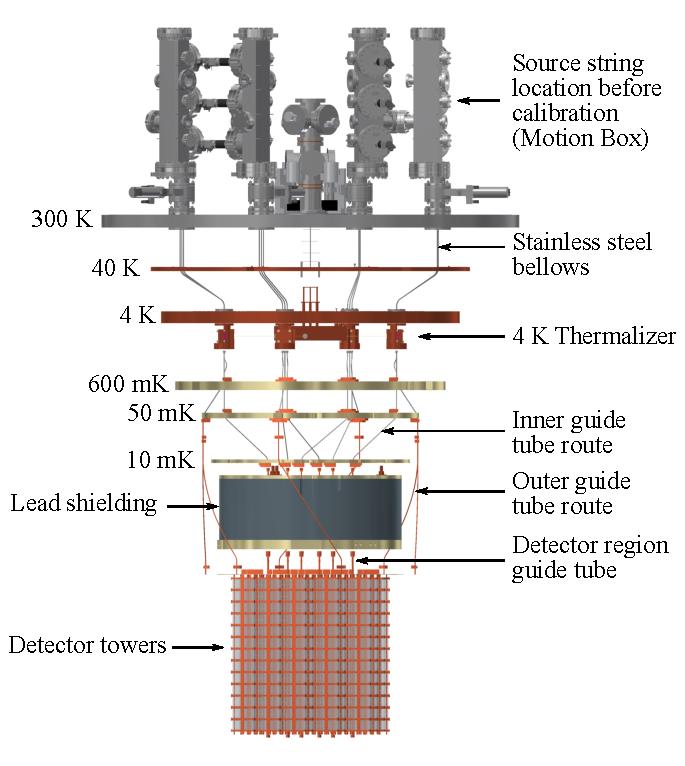
\includegraphics[width=\linewidth]{Figures/DCSintegration.pdf}
\caption[The CUORE Detector Calibration System (DCS)]
{The CUORE Detector Calibration System (DCS).
12 kevlar strings are deployed intermittently into the cryostat through individual tubes through the stages of the cryostat.
6 of the strings are deployed through the inner guide tubes into the 10 mK region of the cryostat between the detector towers, and the other 6 strings are deployed outside the towers in the 50 mK region.
Figure from \cite{Cushman:2016cnv}.}
\label{fig:DCSintegration}
\end{figure}

\section{Calibration Hardware}

The DCS can be divided into a few separate hardware components: the 12 source strings, the set of guide tubes for each string, the 4 motion boxes, the 4-K thermalization system, and the cabling for the software control system.
Each of these sets of components has different technical challenges, particularly for the calibration tubes nearest to the detectors that have stringent radioactivity requirements, and are described in more detail in this section.

\subsection*{Calibration Source Strings}
There are 12 calibration source strings, referred to throughout the section as source strings, that are deployed in to the detector region in order to calibrate the 19 towers of CUORE.
These source strings consist of copper capsules covered in PTFE heat shrink tubing that enclose the 2\% thoriated tungsten source inside, shown in \autoref{fig:source_carrierA}.
The copper is crimped on top and bottom in order to hold it onto the Kevlar string and to hold the source inside, and the PTFE heat shrink reduces the friction between the copper capsules and the DCS guide tubes. In addition, the bottom 8 capsules have reducing spacing and are wider and shorter than the other capsules, shown in \autoref{fig:source_carrierB}.
The mass of the weight capsules (and the Kevlar in between) on the string is 2.8 g, the mass of all 33 capsules (and the Kevlar in between) on a string is 5.6 g, and the mass of an entire unwound string is 13.7 g.
The spacing of the capsules is 6 mm between the weight capsules and PTFE ball and 21 mm between the source capsules.
The decision for the number of source capsules and the relative spacings was optimized based on the need for consistent irradiation over each floor of the CUORE towers and the competing need for minimizing thermal load for cooling purposes, as more capsules would make it easier to uniformly irradiate the towers, but more capsules require more thermalization.
As the sources are deployed into the cryostat under their own weight, these heavier capsules (called ``weight" capsules, opposed to the other ``source" capsules\footnote{Despite the naming convention, all the copper capsules contain radioactive sources.}), and particularly the PTFE guide ball, assist the strings with lowering into the funnels between stages and in detecting obstructed paths.
For example, if the tubes are not perfectly vertically centered, the guide ball will be caught by the funnel and guide the string down into the funnel, where the weight of the capsules will pull the string down into the funnel correctly.
This is opposed to a case where, if there were no weight capsules, some string would fall into the tube, but the rest would drape off the side of the funnel and fail to deploy since the string would not be sufficiently pulled down into the tube.

\begin{figure}[htpb]
\begin{center}
\begin{subfigure}[b]{0.60\textwidth}
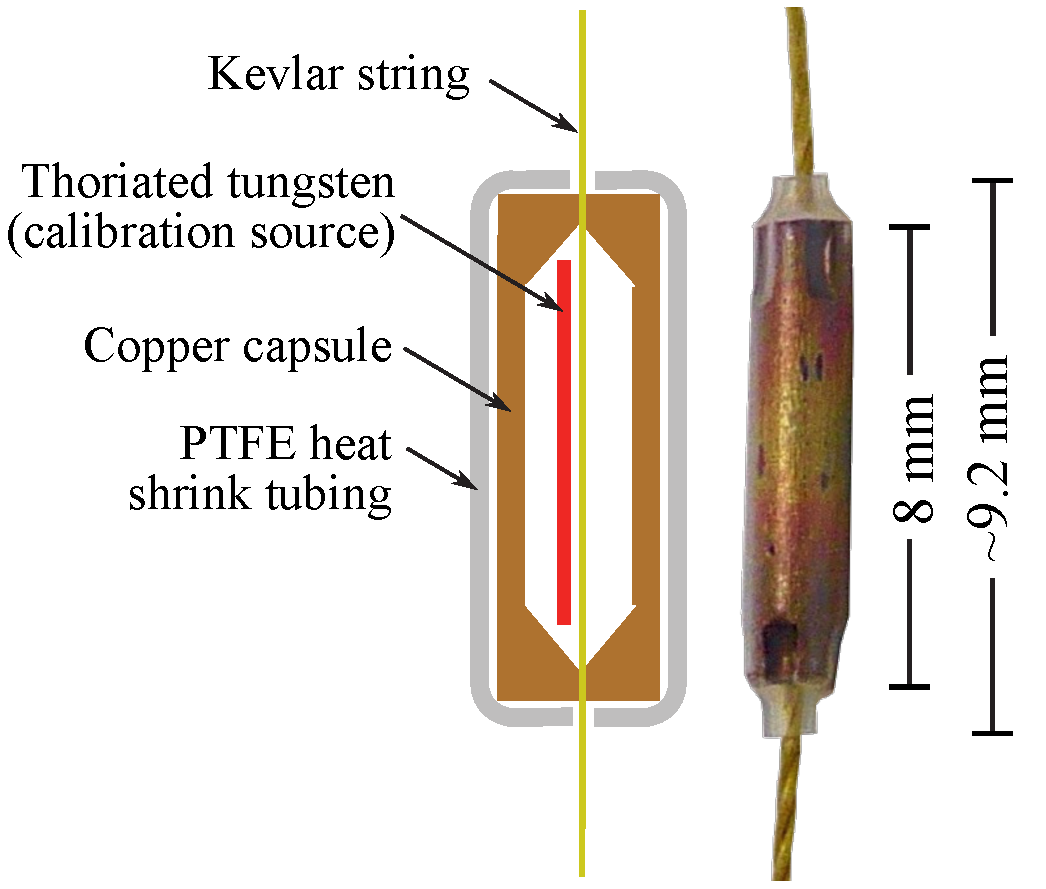
\includegraphics[height=2.2in]{Figures/source_capsule_schematic.pdf}
\caption{}
\label{fig:source_carrierA}
\end{subfigure}
\begin{subfigure}[b]{0.15\textwidth}
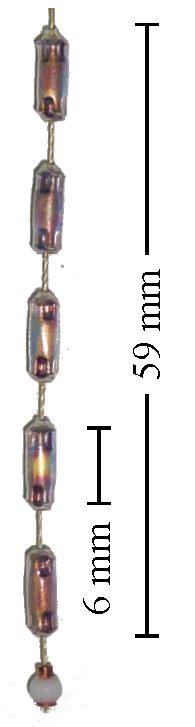
\includegraphics[height=2.7in]{Figures/string_bottom.pdf}
\caption{}
\label{fig:source_carrierB}
\end{subfigure}
\end{center}
\caption[(a) Schematic and photograph of an assembled source capsule. (b) Photograph of five heavier bottom capsules and PTFE ball at the bottom of a source string]{(a) Schematic and photograph of an assembled source capsule. (b) Photograph of five heavier bottom capsules and PTFE ball at the bottom of a source string.}
\label{fig:source_carrier}
\end{figure}
 
Recalling that one of the design goals for the DCS is to calibrate all 988 crystals in as short a time as possible, the strings are configured, when fully deployed in the cryostat, to optimize coverage on all the crystals, as the time it takes to calibrate the detector array is limited by the time it takes the least-irradiated crystals to calibrate.
To this end, the final positions of the source strings are configured in a double-hexagonal pattern, as shown in \autoref{fig:Calibration_source_top_view} with the inner source strings inside the 10-mK vessel irradiating the towers and floors closest to the center and the outer strings outside the 50-mK vessel irradiating the towers and floors furthest from the center.
The inner source strings are located about 2 cm from the faces of the crystals, and the outer source strings are about 18 cm away from the crystals, although they are shielded from the crystals by the 10-mK and 50-mK vessel.
As a result of this geometry, there are two main differences between the copper capsules in each source string and between the inner and outer strings, viz., the bottom and top capsules of each string have a boosted activity relative to the capsules in the middle of the string, and the capsules in the outer strings have a boosted activity relative to their counterparts in the inner strings, with the specific activities of each described in \autoref{tab:calibration_activities}
In addition, there is one more capsule on the inner strings relative to the outer strings, which is due to the fact that when the strings were made, the activities were lower than anticipated and needed a more significant boost at the top capsules of the source string.
The reason for this asymmetry for the activity of the capsules on each string is to have roughly equal rates on each crystal on each floor, and, since the source strings are only slightly longer than the towers themselves\footnote{The inner and outer calibration strings have an active region 80 and 83 cm long, respectively, while the towers are 76 cm from the bottom frame to the top frame of the tower.}, these edge effects need to be considered for optimal calibration.
The spacing of the source capsules is designed such that each floor sees roughly 2-3 adjacent capsules at a time, and the vertical geometry of the strings in their nominal vertical positions is shown in \autoref{fig:Calibration_source_tower}.

\begin{figure}[htpb]
\begin{center}
\begin{subfigure}[b]{0.5\textwidth}
    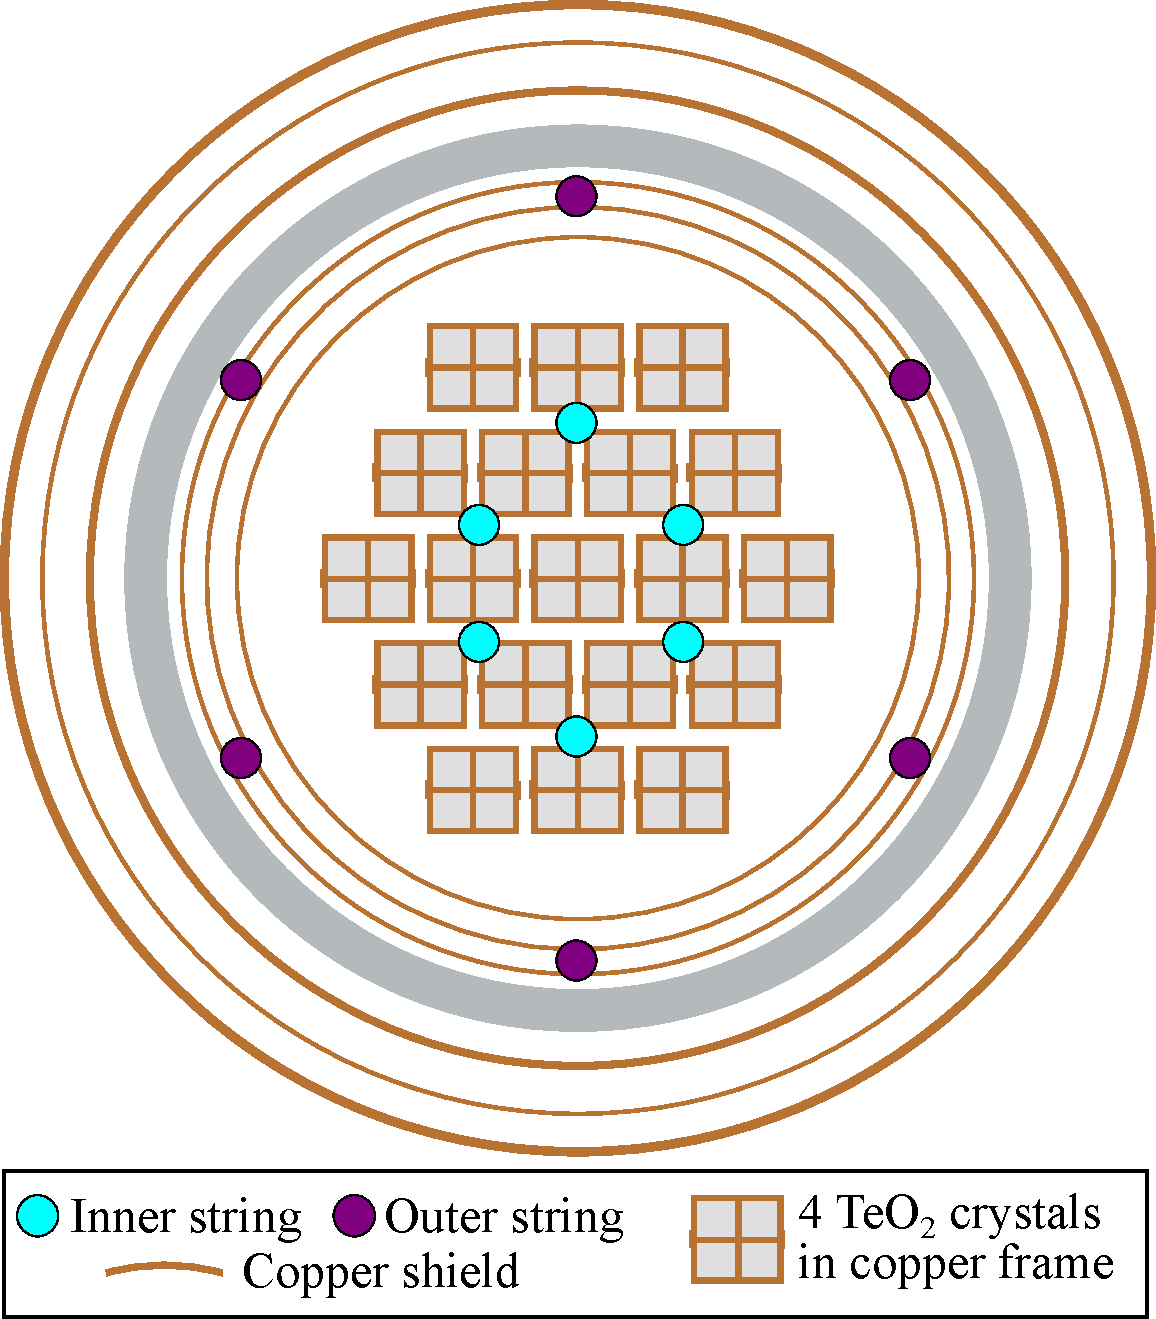
\includegraphics[height=3.25 in]{Figures/CUORE_calibration_location.pdf}
    \caption{}
    \label{fig:Calibration_source_top_view}
\end{subfigure}
\begin{subfigure}[b]{0.40\textwidth}
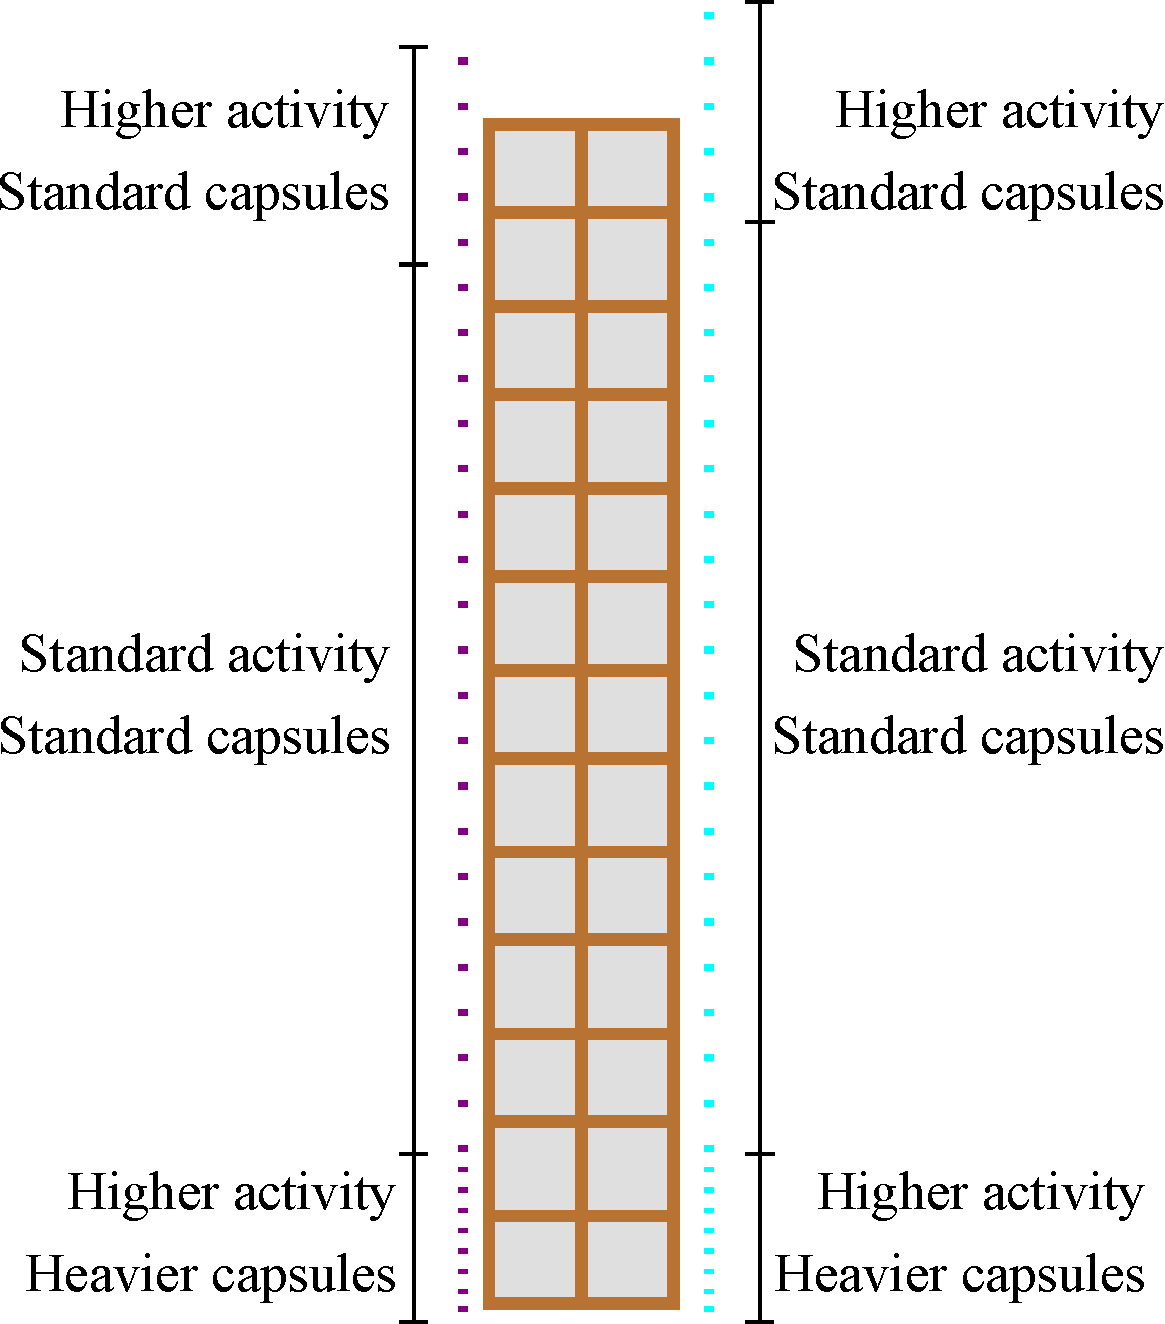
\includegraphics[height = 3.5 in]{Figures/Cuore_tower_calibration.pdf}
\caption{}
\label{fig:Calibration_source_tower}
\end{subfigure}
\end{center}
\caption[(a) A top-down schematic of the calibration source strings in the cryostat.
(b) A side-view schematic of an inner and outer calibration string next to a tower]
    {(a) A top-down schematic of the calibration source strings in the cryostat.
    The inner strings irradiate the innermost towers, and the outer strings irradiate the outermost towers.
    Due to space constraints, the outer sources are located outside the 50-mK vessel.
    (b) A side-view schematic (horizontal axis not to scale) of a tower with an adjacent inner (right) and outer (left)  calibration string.
    Figures adapted from \cite{Cushman:2016cnv}.}
\label{fig:Calibration_source_locations}
\end{figure}

\begin{table}[htbp]
    \centering
    \caption[The number of capsules and activities of each calibration source]
    {The number of capsules and activities of each calibration source.
    The capsules are listed from bottom to top, with the 8 capsules corresponding to the weight capsules on the string.
    For the activity, the activity of each capsule is listed, along with the total summed activity of that component.
    In total, the activity of the inner strings is 3.6 Bq, and the activity of the outer strings is 19.4 Bq, with the activities listed as the activity of the $^{208}$Tl decay in the $^{232}$Th decay chain.}
    \label{tab:calibration_activities}
    \begin{tabular}{lccc}
    \hline 
    \hline
        String type & Capsules & Activity (Bq) & Summed Activity (Bq) \\
        \hline 
        \multirow{3}{*}{Outer} & 8 & 0.64 & 5.12 \\
        & 20 & 0.48 & 9.52 \\
        & 5 & 0.95 & 4.75 \\
        \hline
        \multirow{4}{*}{Inner} & 8 & 0.07 & 0.54 \\
        & 21 & 0.09 & 1.95 \\
        & 4 & 0.08 & 0.31 \\
        & 1 & 0.80 & 0.80 \\
        \hline
        \hline
    \end{tabular}
\end{table}

\subsection*{Motion Boxes}
On top of the cryostat and mounted on the 300-K plate, there are four stainless steel motion boxes, with dimensions $12.6\times7.9\times60.7~\textrm{cm}^3$ shown in \autoref{fig:motion_box}, that contain the DCS calibration strings while they are not being deployed and the motors that control the motion of the strings.
\begin{figure}[htpb]
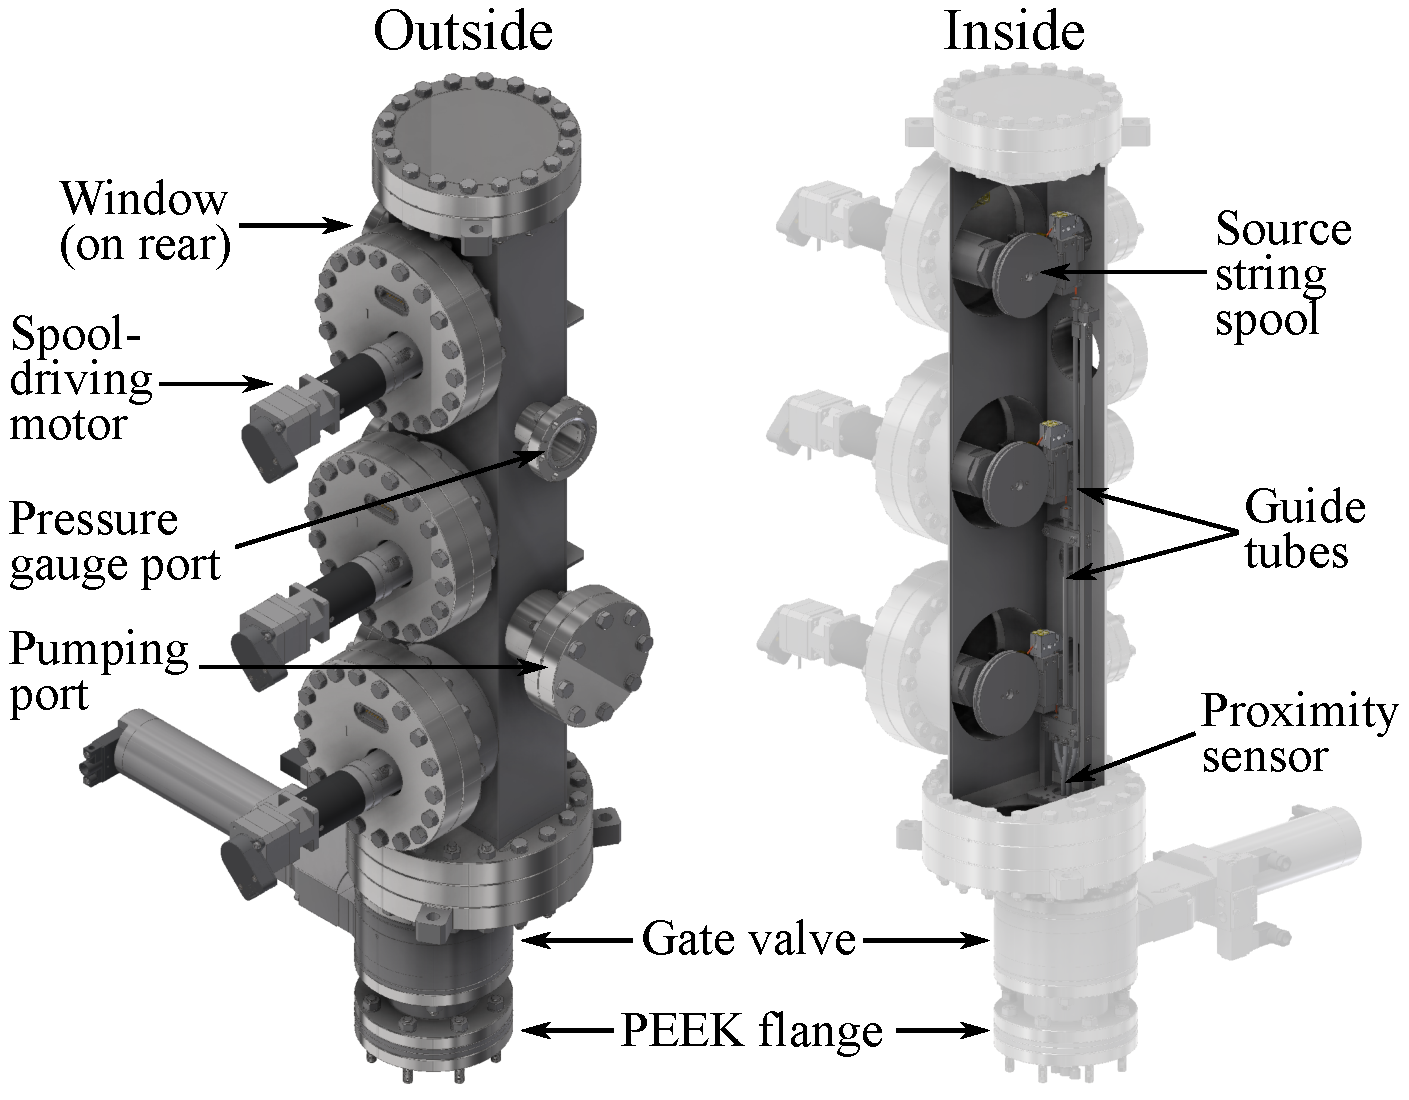
\includegraphics[width=0.9\linewidth]{Figures/motion_box.pdf}
\caption[A rendering of a single motion box from two different angles]
{A rendering of a single motion box from two different angles. The motion box is mounted vertically with the PEEK flange on top of the cryostat with the three source strings spools above. The windows on each motion box allow for the source strings to be observed from outside.}
\label{fig:motion_box}
\end{figure}
The motion boxes are electrically isolated from the rest of the cryostat by a polyetheretherketone (PEEK) flange in order to prevent ground loops, with the gate valves that connect the motion boxes to the IVC above them.
Above the gate valve and inside the motion box is a proximity sensor that detects when the copper capsules enter and disturb the electromagnetic field produced by the sensor.
This allows for us to determine when individual source capsules or the weight capsules\footnote{The sensor is unable to resolve the denser-packed weight capsules and triggers continuously while they are in the sensor.} move either into or out of the motion box.
Above this, 3 conflat flanges seal the 3 drive spools to the motion box and are shown in \autoref{fig:drive_spool}.
\begin{figure}
    \centering
    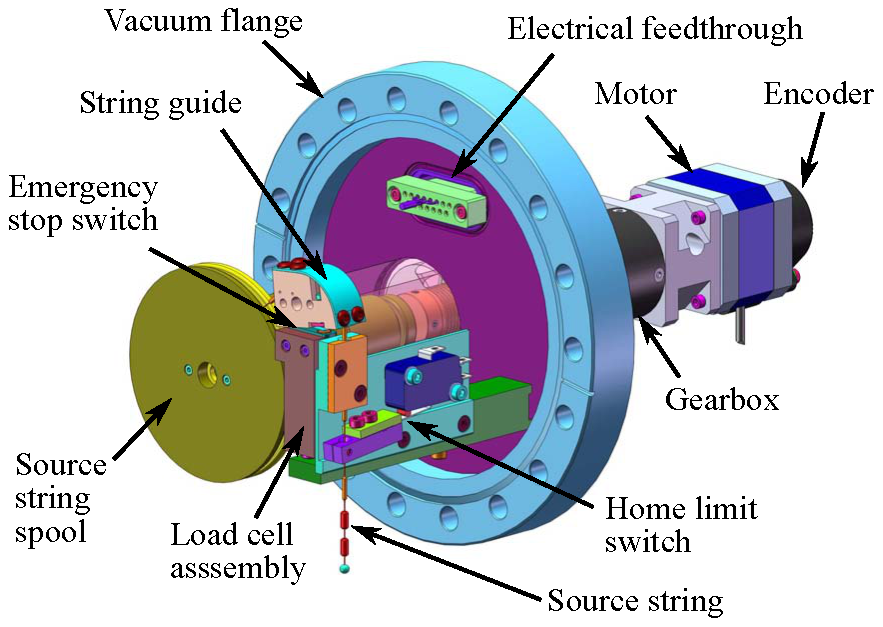
\includegraphics[width=0.8\linewidth]{Figures/drive_spool.pdf}
    \caption[The drive spools inserted into the DCS Motion Boxes]
    {The drive spools inserted into the DCS Motion Boxes.
    These spools contain the hardware used for deploying and extracting the strings and many of the sensors used for monitoring the system and providing interlocks.
    Not shown on the diagram are heat sinks which are mounted behind the encoder.}
    \label{fig:drive_spool}
\end{figure}
On these drive spools, a stepper motor\footnote{Kollmorgen CTP11ELF11MMA00 \url{http://sine.ni.com/nips/cds/view/p/lang/en/nid/203936}} drives a rotary feedthrough\footnote{\url{https://www.mdcvacuum.com/DisplayPartResp.aspx?d=MDC&p=652000}} to turn the source string spool and is used to raise and lower the strings into the cryostat.
With this stepper motor, it takes 200 steps for a full revolution, and in conjunction with a 320:1 reducer, takes 64,000 steps for a full rotation of the source string spool.
Behind the motor is an encoder\footnote{\RaggedRight\url{https://www.usdigital.com/products/encoders/incremental/rotary/kit/E5-1000-197-IE-D-D-G-B}} that optically measures the rotations of the motor and acts to double-check that the steps sent to the stepper motor are properly implemented.
This is critically important as having precise knowledge of the string position enables us to use the 4-K thermalizers, which are discussed later, and is one of the few ways we have information about the strings while they are in the cryostat.
The last component outside of the motion box vacuum is a thermal fin mounted on the back of the encoder.
As the motor heats up during operation to temperatures of over 325 K, this fin assists with cooling the motor body, and reduces the temperature in operation to be 310 K.
This helps another component on the drive spool in the interior of the motion box, the load cell\footnote{\url{https://www.smdsensors.com/products/type/s251-miniature-platform-load-cell/?highlight=251\%20}}.
This load cell is rated up to 20 N and is used to measure the tension on the string.
This is another critical component of the system, as the measurement of the tension is the only signal that a source string has encountered difficulties during deployment or extraction, e.g. the tension rises if the string is obstructed on the way up and decreases if the string misses a funnel and is spooling up on one of the cryostat plates.
However, a known issue with load cells is that they have significant thermal drift, which the thermal fin helps mitigate.
The load cell is read out through an electrical feedthrough on the spool and the output signals are filtered, amplified, and digitized.
The last two components on the drive spool are used for interlocks on the system.
The home limit switch is lever with a hole sized to allow source capsules but not weight capsules through.
When the weight capsules attempt to pass up through the lever, it triggers the switch and allows for the the string to stay partially unwound from the spool, in addition to being the position that the source strings are left between calibrations.
The last component on the drive spool is a PTFE guide that connects to a microswitch that triggers when the tension in the string becomes too high, around 0.5 N.
This switch is not used during normal operation of the DCS, but activates in the case that the string becomes caught while extracting and experiences a rapid rise in tension that an operator cannot react quickly enough to.
In addition, this interlock directly shuts down the hardware that runs the motor and kills any motion, protecting the string in the case of user or software error.
A useful tool that an operator can use on the motion box are the windows that open on the opposite face of the motion box from the drive spools. These spools allow the operator to see the string coming out of the PTFE string guide and into the home switch and to verify string integrity and motor operation even when the motion box is closed off and under vacuum.
When the source strings are deployed into the cryostat, they are each contained in a separate guide tube that guides them through the motion box and down into the proximity sensor and below, with a gap at the gate valve.
Lastly, two of the four motion boxes are instrumented with a vacuum gauge, as each motion box is its own vacuum environment, only connecting to the IVC when the gate valves are opened, such as when the calibration strings are being deployed into the cryostat.
The full vacuum setup of the motion boxes is shown in \autoref{fig:vacuum_setup_diagram}.
Before operation of the DCS, the motion boxes are first pumped out to a pressure of $\mathcal{O}(10^{-5})$ mbar before opening the gate valves into the cryostat.
During operation of the DCS, the motion boxes are continuously pumped by the OVC turbo, until the strings are fully deployed into the cryostat.
Afterwards, the hand valves on the motion boxes are closed and the motion boxes are cryopumped through the tubes below the gate valve into the IVC\footnote{Unfortunately, this is a significant design flaw of the vacuum system of the experiment, as any leak or outgassing in the motion box builds up in these tubes and can fully block a calibration string's movement.}.
This cryopumping can be observed as well as shown in \autoref{fig:capsule_cryopumping} when the cold capsules are extracted from the cryostat and return to the motion box.

\begin{figure}[htbp]
    \centering
    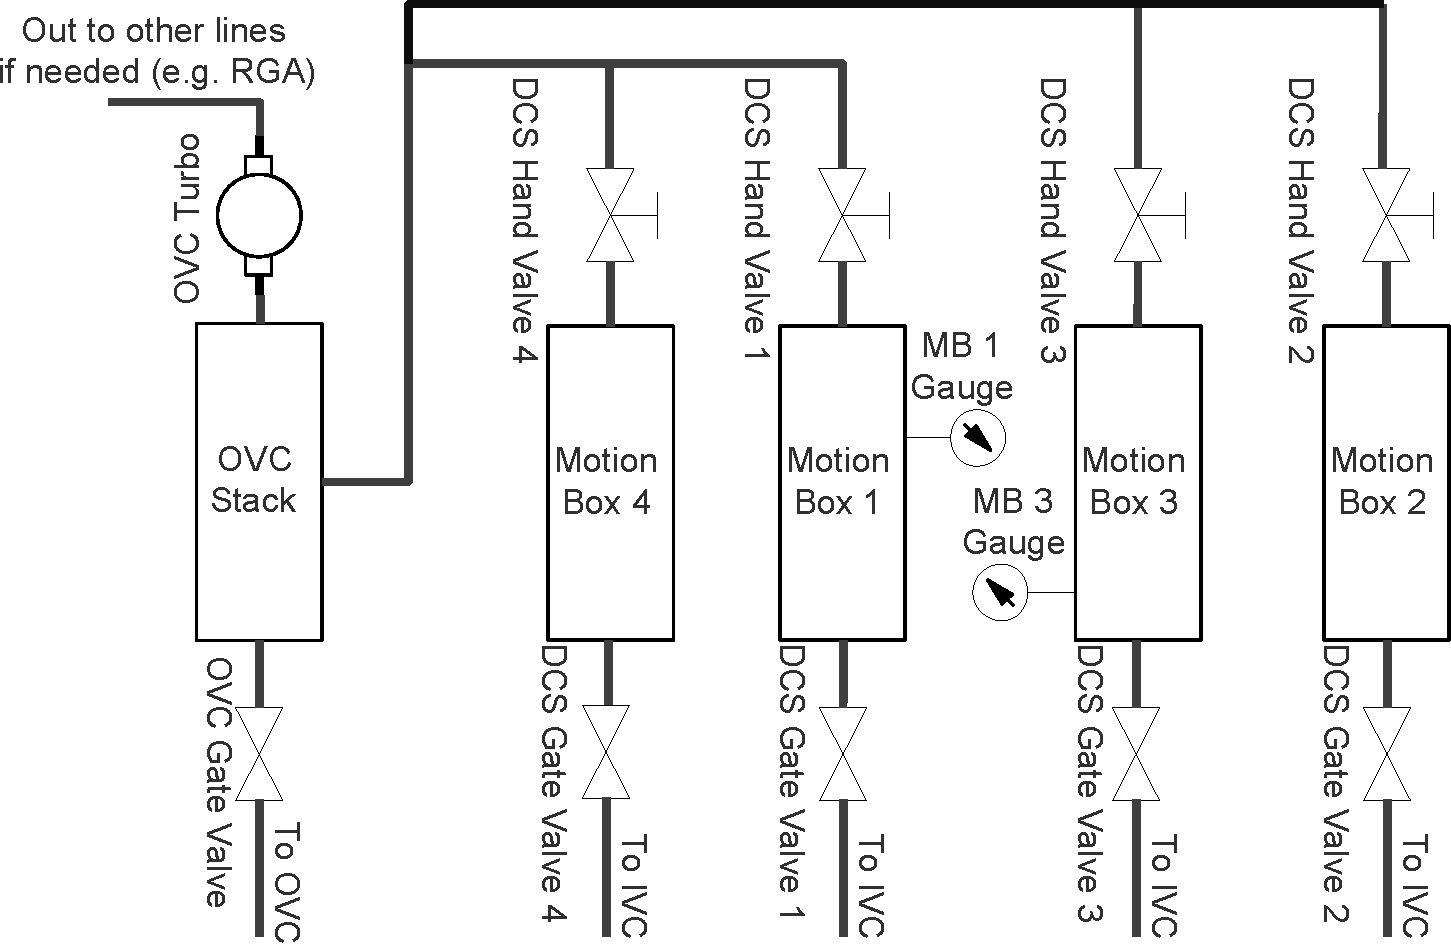
\includegraphics[width=0.9\linewidth]{Figures/DCS_Vacuum_System_Edit.pdf}
    \caption[A schematic of the vacuum system of the DCS]
    {A schematic of the vacuum system of the DCS.
    The motion boxes are separated by a hand valve from the OVC stack and can be pumped out with the OVC turbo pump.
    There are two main lines of KF-50 bellows extending from the OVC that connect to two motion boxes independently.
    Each of these sets of motion boxes has its own vacuum gauge, and each have a gate valve that connects them to the IVC.}
    \label{fig:vacuum_setup_diagram}
\end{figure}

\begin{figure}
    \centering
    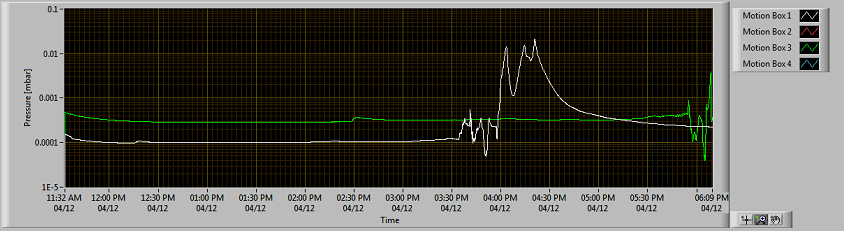
\includegraphics[width=0.9\linewidth]{Figures/CUORE_vacuum_cryopumping.png}
    \caption[The pressure in the motion boxes when cold capsules are extracted into the room-temperature motion boxes]
    {The pressure in the motion boxes when cold capsules are extracted into the room-temperature motion boxes.
    Starting at 3:30 pm, it can be seen that the capsules cryopump the motion box when they arrive, and then the gas that had previously frozen onto the capsules melts and evaporates back into the motion box.}
    \label{fig:capsule_cryopumping}
\end{figure}

\subsection*{Guide Tubes}
\label{ssec:Guide Tubes}
When the strings are deployed down into the cryostat out of the motion boxes, they are guided down through a series of guide tubes, shown in \autoref{fig:DCSintegration} and \autoref{fig:dcs_thermal_coupling}.
At the 300-K stage, the strings first are guided by an ``s-tube" that connects the tube from the 300-K stage down to the 4-K thermalizers, which are discussed later in \autoref{ssec:Thermalization_and_Thermometry}, and are shown in \autoref{fig:s-tube}.
\begin{figure}[htbp]
    \centering
    \includegraphics[height=0.5\pageheight]{Figures/s_tube_labeled.pdf}
    \caption[The 3 stainless steel s-tubes below a motion box]
    {The 3 stainless steel s-tubes below a motion box.
    The tubes are thermally connected to the 300-K, 40-K, and 4-K plates and form a thermal gradient between each.
    The bend in the tubes is for both geometrical reasons and for reducing the radiative heat load on the bottom stages of the cryostat as there is no line-of-sight from the top of the funnels at 300-K to the bottom at 4-K.
    As the strings are deployed down through the tube, they are thermalized by contact with the walls of the tube and by radiative cooling.
    Figure from \cite{Cushman:2016cnv}.}
    \label{fig:s-tube}
\end{figure}
Below the s-tubes and the 4-K thermalizers are the stainless steel 600-mK guide tubes, shown in \autoref{fig:600mK_guide_tubes}.
It is at this stage that the first differences between the inner and outer guide tubes appear.
As the inner source strings will be deployed into the 10-mK region of the cryostat, they require more thermalization, but, due to geometrical constraints within the cryostat, the path between the 600-mK and 50-mK stages for the inner strings is vertical, which reduces the ability of the tubes to extract heat from the capsules.
As shown in \autoref{tab:cryostat_cooling_power}, the cooling power of the cryostat drastically decreases at colder stages; therefore, the inner guide tubes have a chicane just under their funnel that assists with the cooling of the capsules by increasing their contact as they pass through the tube.
Under the 600-mK plate, the outer guide tubes take the outer strings to the outside of the 50mK plate, while the inner guide tubes, as noted before, continue straight down through the 50-mK plate.
\begin{figure}[htbp]
\centering
\begin{subfigure}[t]{0.37\textwidth}
\centering
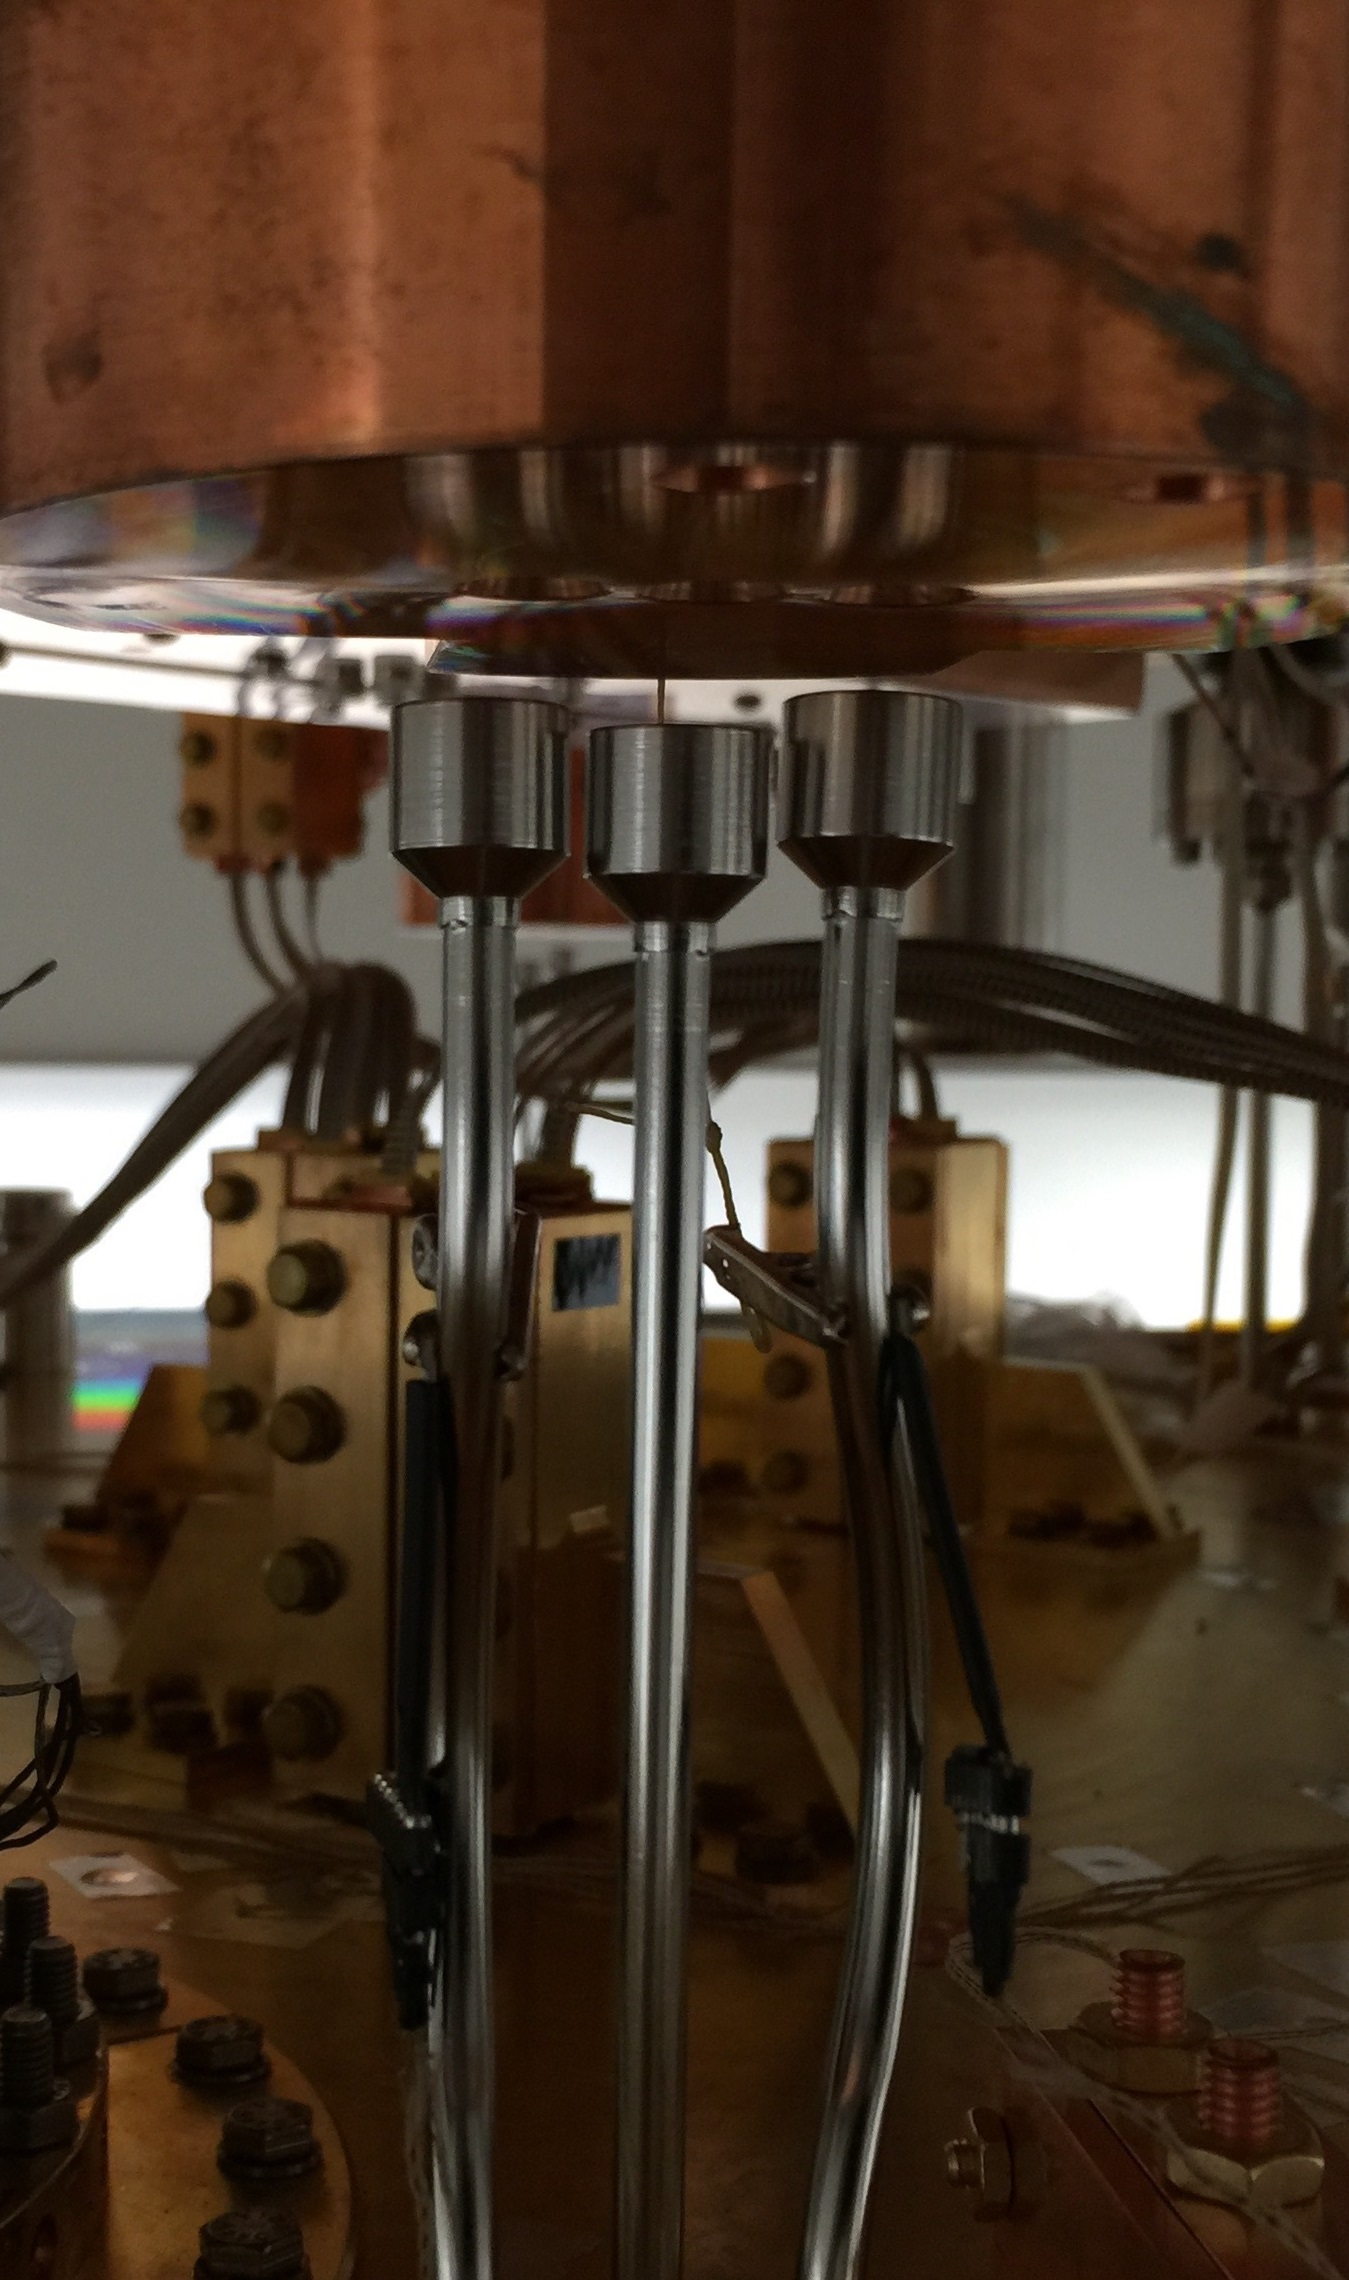
\includegraphics[width=0.9\textwidth, height= 3 in, keepaspectratio]{Figures/600mKguidetube_cropped.jpg}
\caption{}
\label{fig:600mk_guide_tubes_top}
\end{subfigure}
\qquad
\begin{subfigure}[t]{0.5\textwidth}
\centering
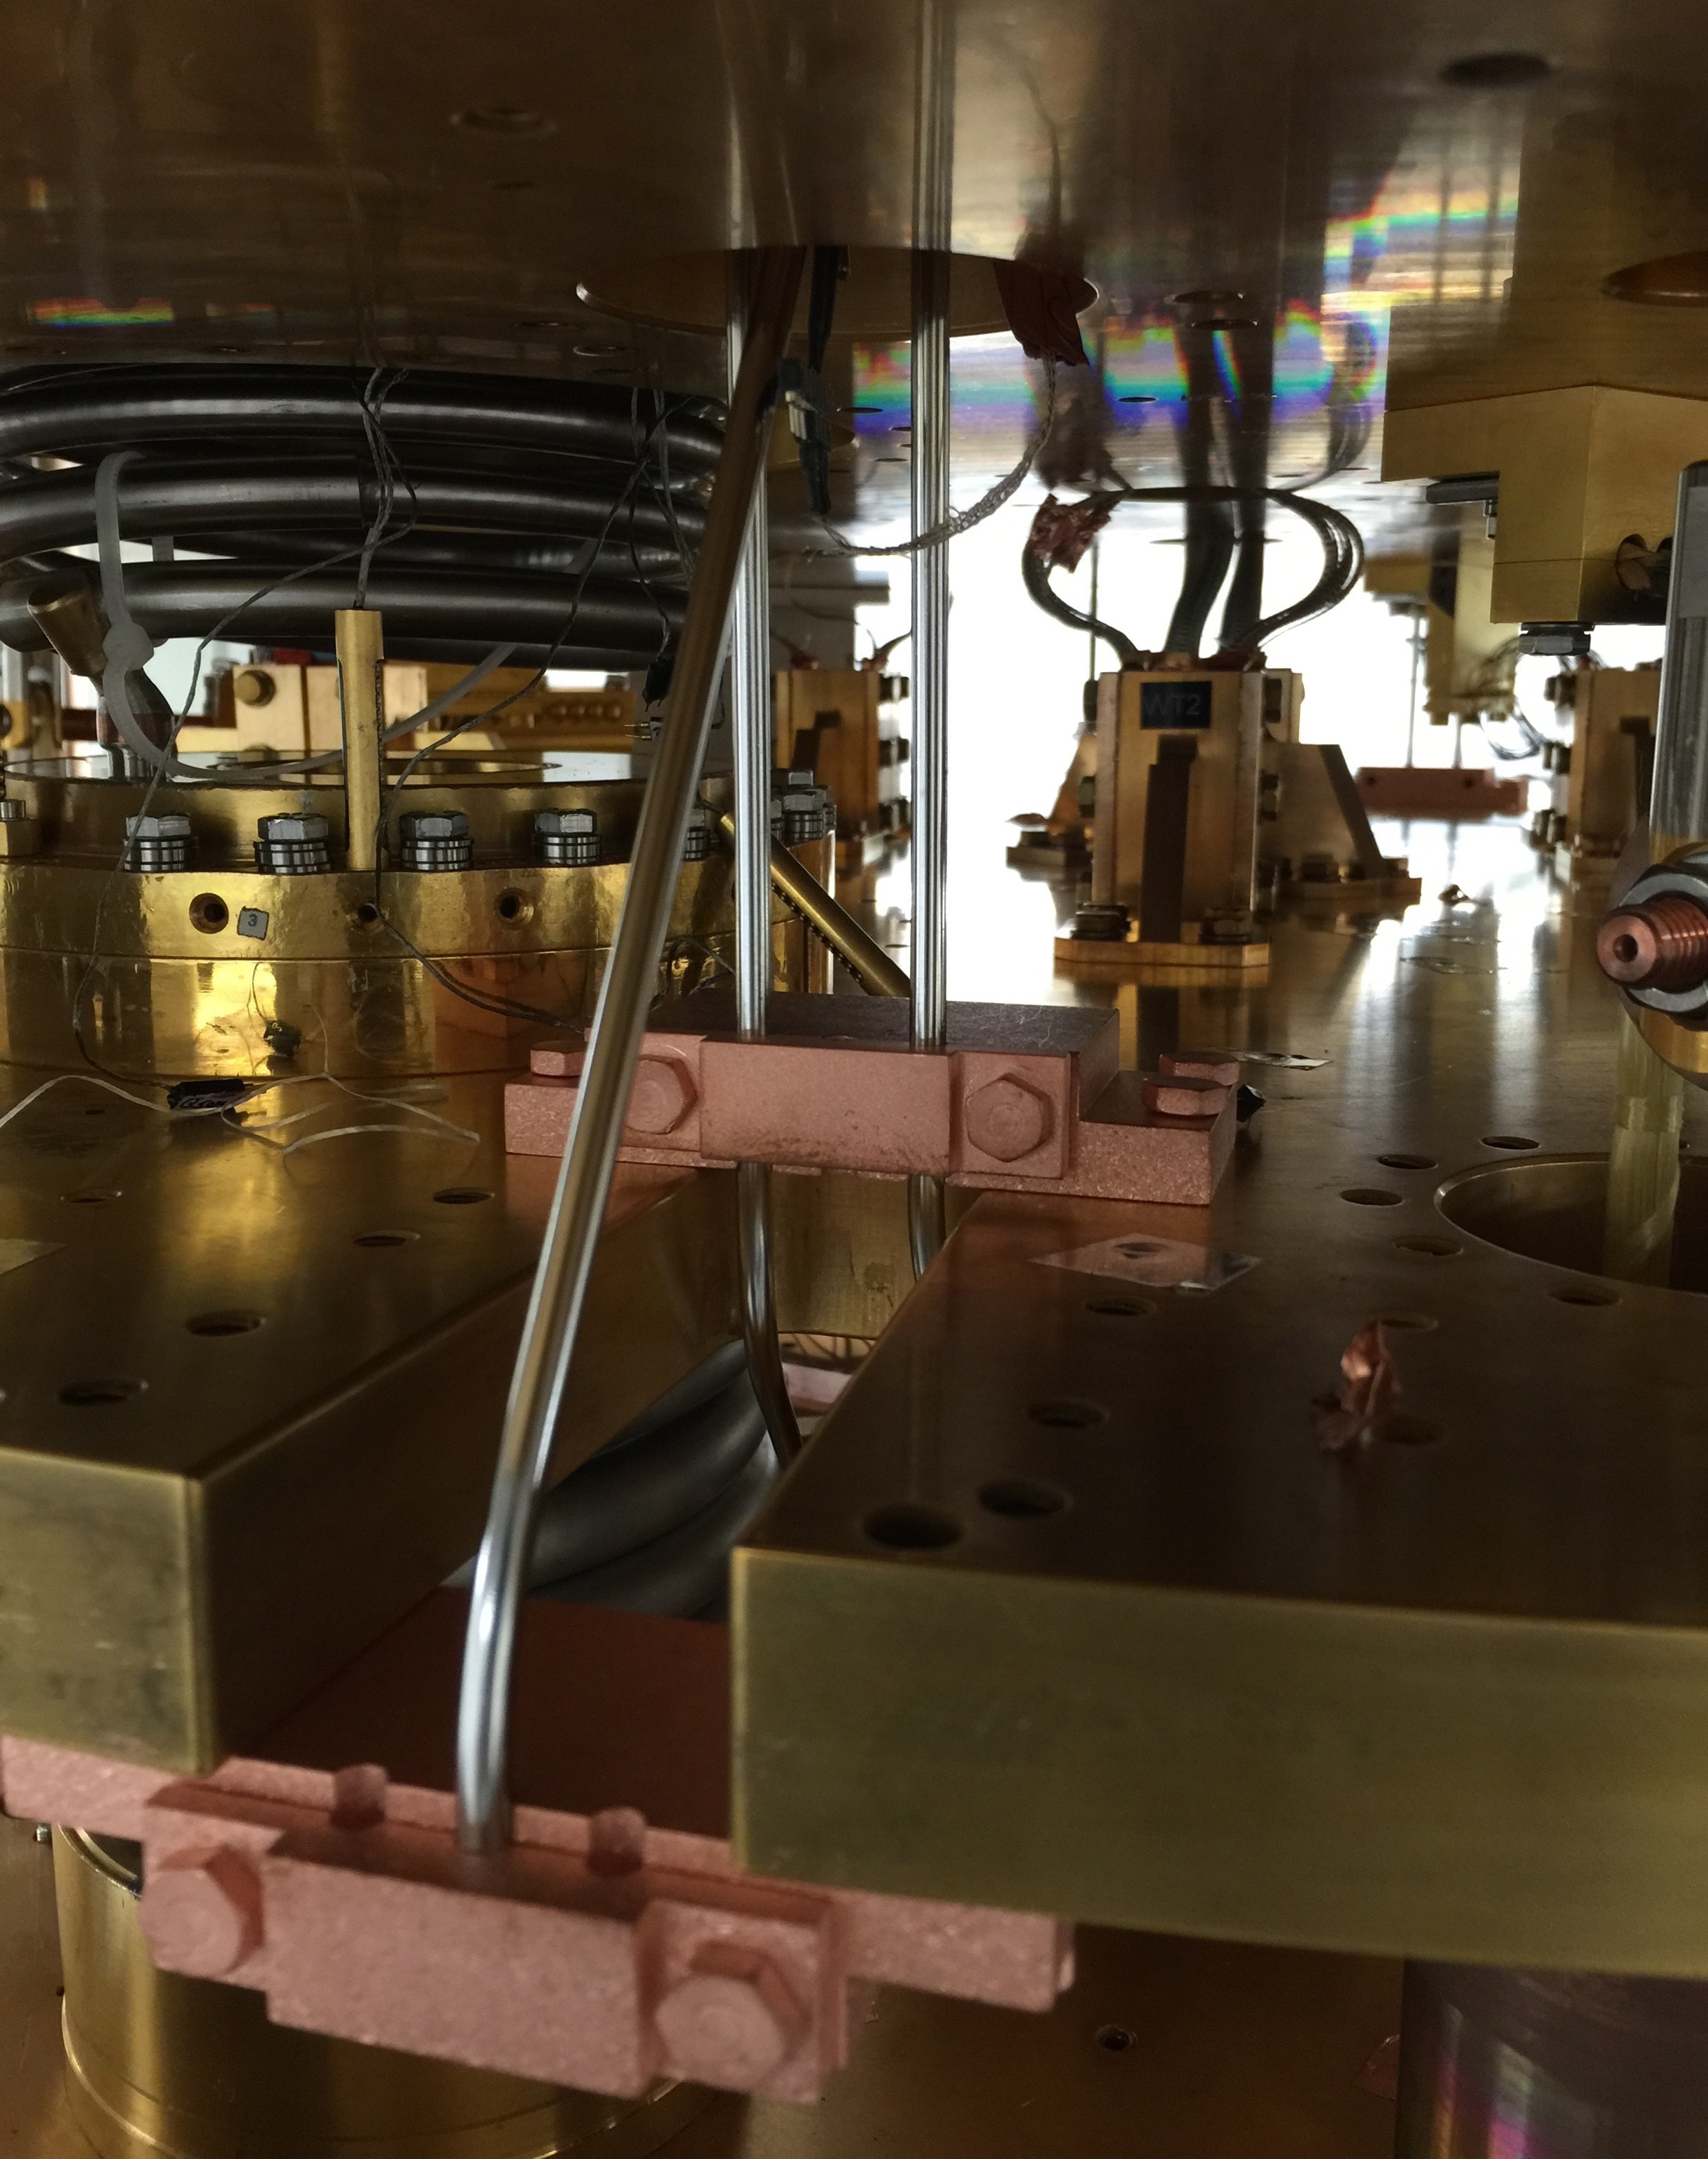
\includegraphics[width=0.9\textwidth, height = 3 in, keepaspectratio]{Figures/600mKguidetube_below_cropped.jpg}
\caption{}
\label{fig:600mk_guide_tubes_bottom}
\end{subfigure}
\caption[Photographs of a set of 600-mK guide tubes above (a) and below (b) the 600-mK plate]
{Photographs of a set of 600-mK guide tubes above (a) and below (b) the 600-mK plate.
In order to safely and reliably catch the strings as they come out of the 4-K thermalizer, top of (a), the funnels for the tubes are significantly wider than the tubes themselves.
The tubes for the inner strings have a chicane that increases the thermal contact between the copper capsules and the guide tube.
Below the 600-mK plate (b), the outer string guide tube path goes out to the outside of the 50-mK shield.
For each of the tubes, they are clamped and thermalized to the 600-mK and 50-mK plates.}
\label{fig:600mK_guide_tubes}
\end{figure}

For the outer guide tubes, the next components are the 6 copper helical tubes around the 50-mK vessel, shown in \autoref{fig:helical_tubes}.
These tubes take the outer strings to their final locations on the outside of the 50-mK vessel.
When the string is fully deployed, the active region of the string hangs freely out of the helical tubes in order to reduce the mass of copper and the resultant radioactive background contributions.
\begin{figure}[htbp]
    \centering
    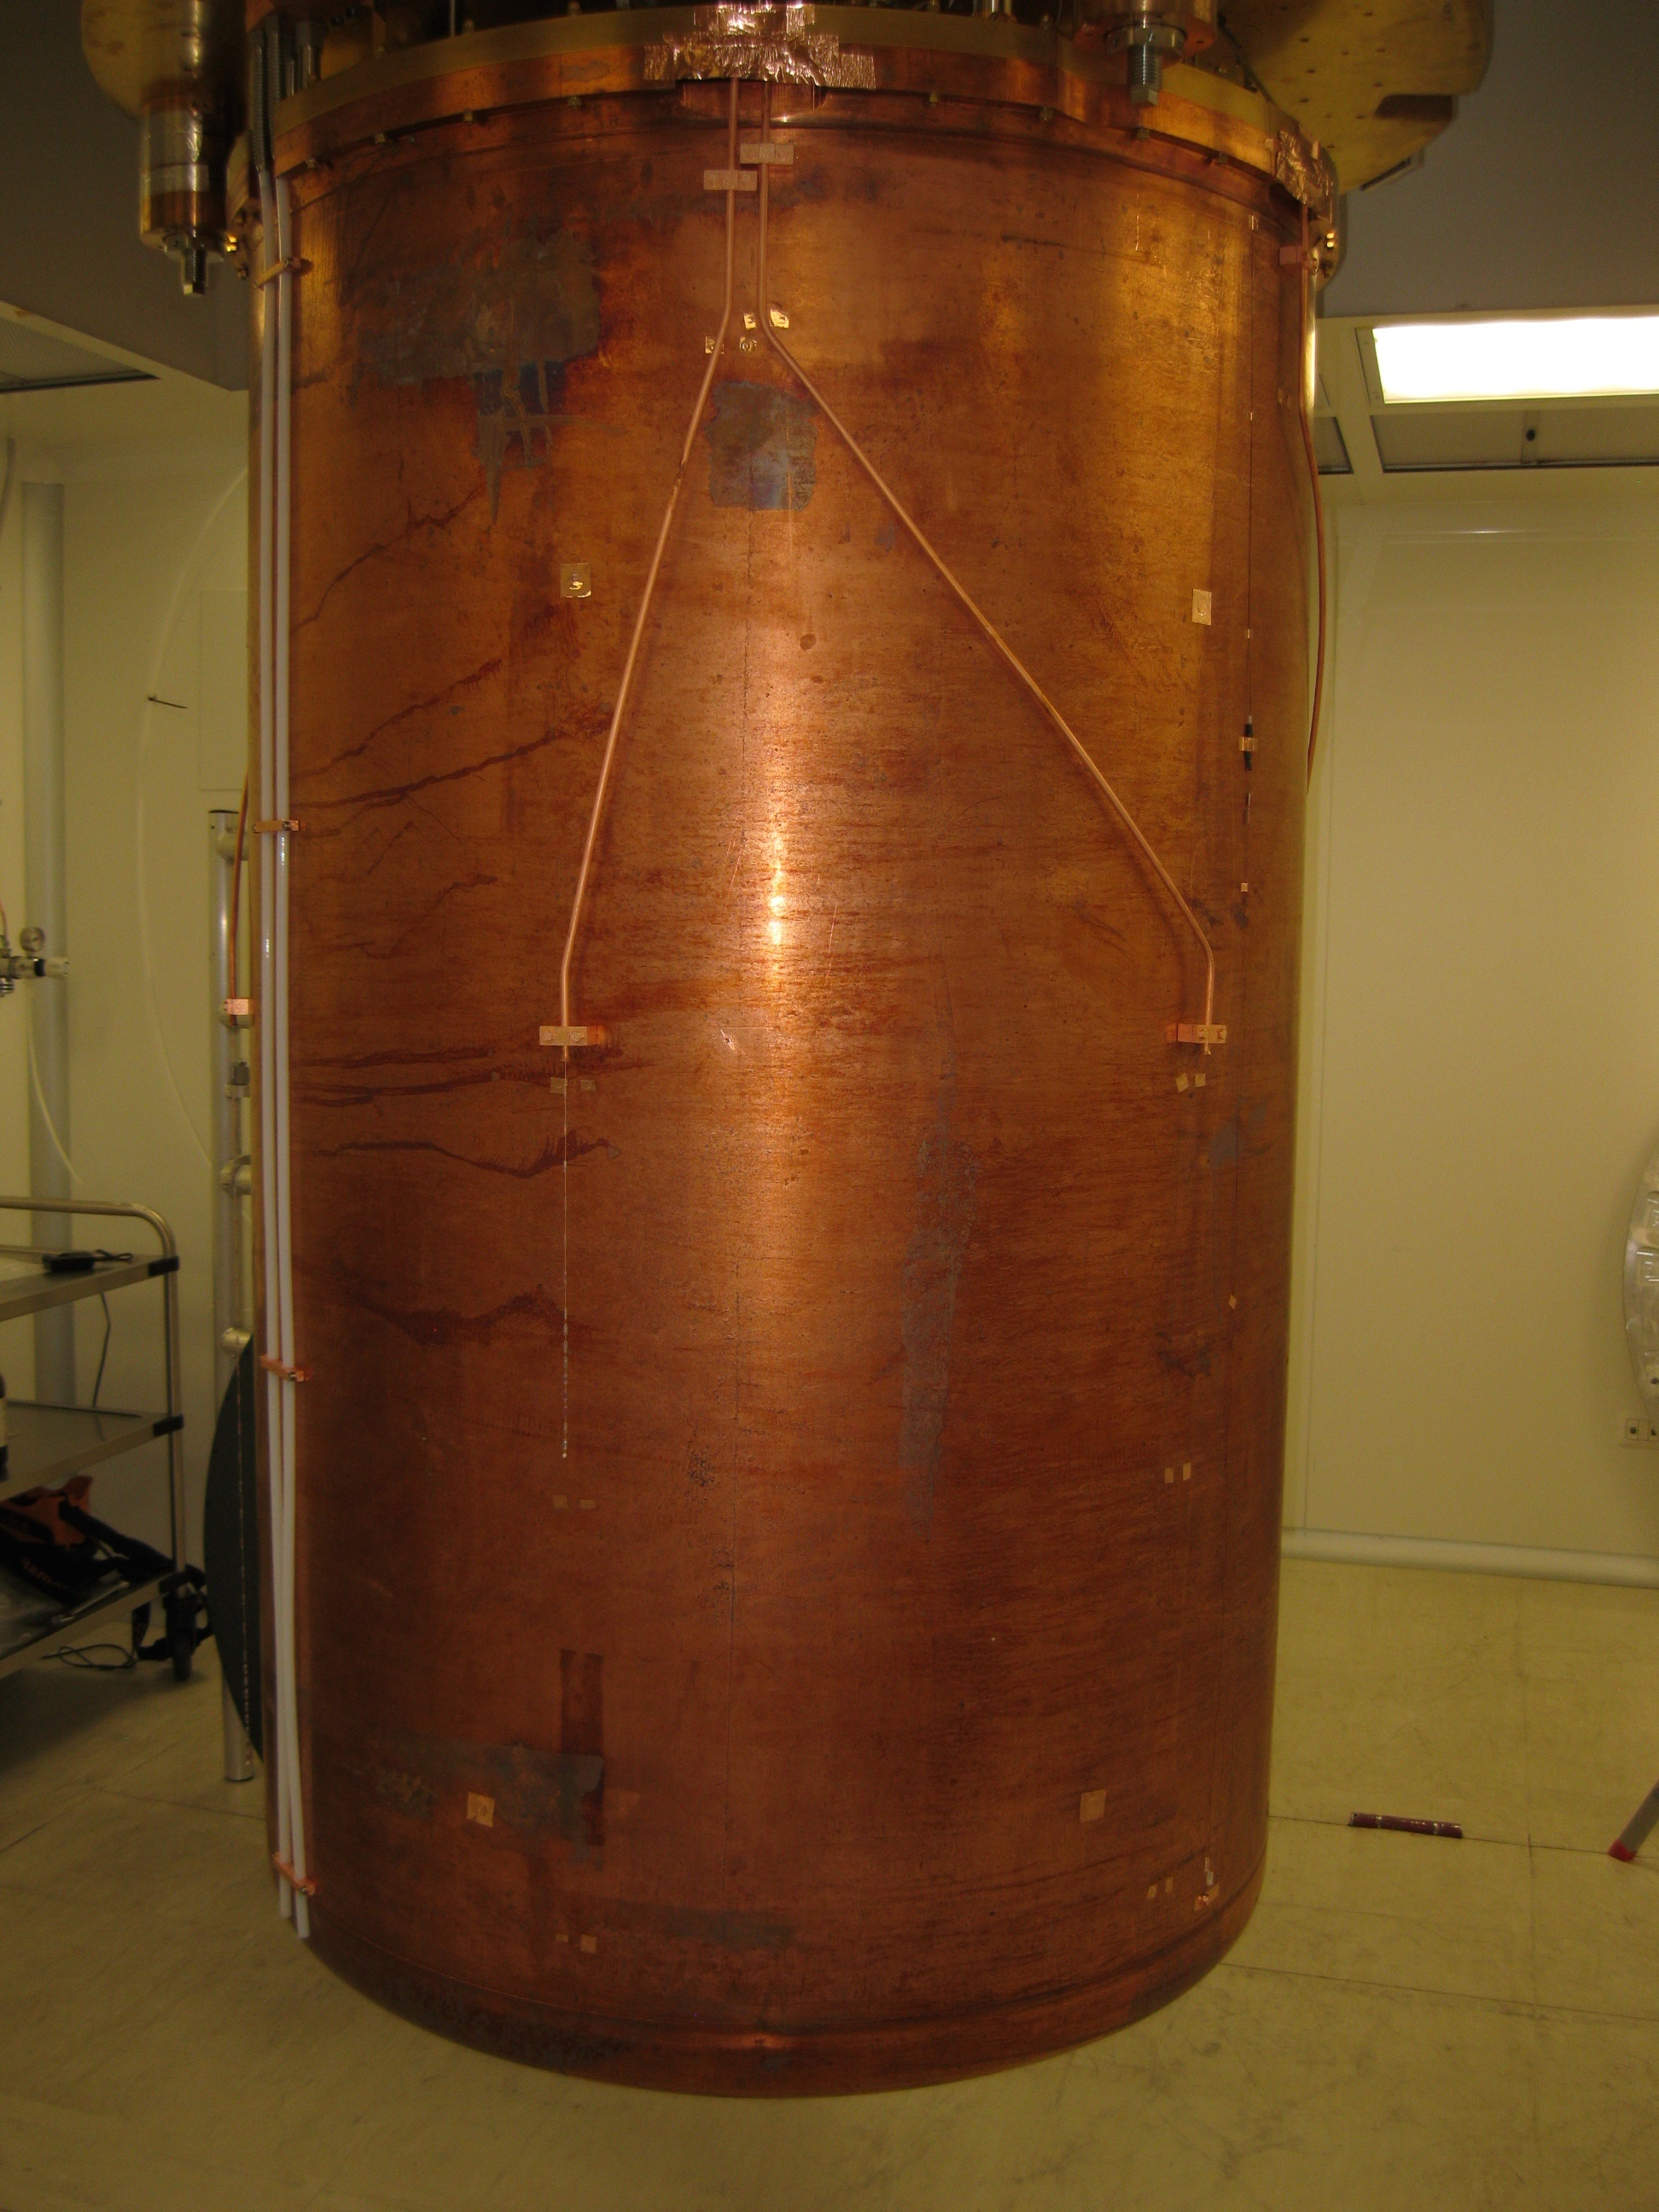
\includegraphics[height = 3.5 in]{Figures/HelicalTubes.jpg}
    \caption[A photograph of two of the helical guide tubes around the 50-mK vessel]
    {A photograph of two of the helical guide tubes around the 50-mK vessel.
    The helical tubes are arranged around the cryostat in such a way as to have the final positions of the outer strings as shown in \autoref{fig:Calibration_source_locations}.
    When fully deployed, the end of the string extends down to a few cm above the bottom of the vessel, and a string can be seen partially hanging out of the left tube.}
    \label{fig:helical_tubes}
\end{figure}

For the inner guide tubes below the 50-mK plate, there is another non-vertical section as the strings are directed towards the center of the tower array and line up with their final positions as noted in \autoref{fig:Calibration_source_locations}.
This section between the 50-mK and the 10-mK plates, is the last non-vertical section of the guide tubes, and is the last chance for thermalization of the strings before reaching the detectors themselves.
Below the 10-mK plate, there are guide tubes in the top lead shield that carry the strings down to the TSP above the detectors. 
In these regions below the 10-mK plate, the guide tubes consist of NOSV copper, and the detector region tubes, since they are hanging near the detectors under the top lead, are cleaned with the procedures mentioned in \autoref{ssec:Parts Selection and Cleaning}.
These detector region guide tubes are made of 3 separate sections and are assembled in a glove box before installation and are installed along with the detectors into the cryostat.

\begin{figure}[htbp]
    \centering
    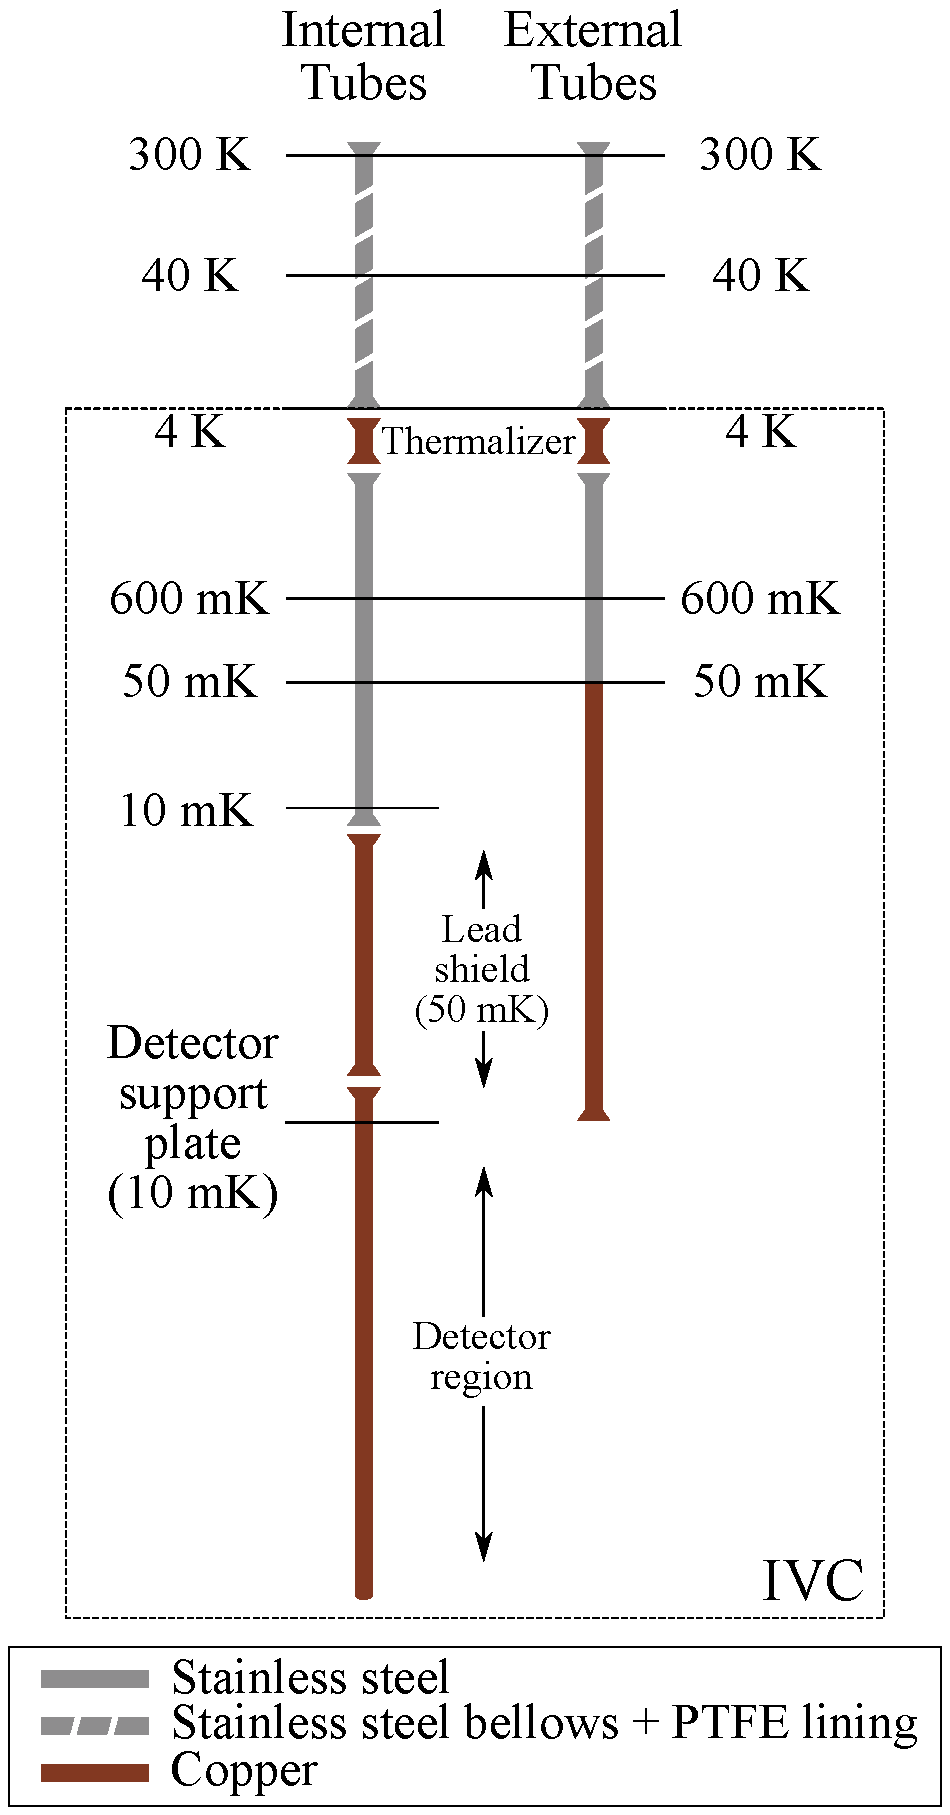
\includegraphics[height=0.4\paperheight]{Figures/thermal_coupling.pdf}
    \caption[A diagram showing the thermal couplings of the DCS tubes for both the internal and external sources]
    {A diagram showing the thermal couplings of the DCS tubes for both the internal and external sources.
    In order to minimize the thermal load on the cryostat, there are multiple breaks in the DCS tubes with funnels for the calibration sources to pass through.
    Near the detectors, the tubes switch from being stainless steel with low thermal conductivity to low-background copper.
    For the external tubes, there are no tubes below the lead shield and the source capsules hang freely.
    Figure from \cite{Cushman:2016cnv}.}
    \label{fig:dcs_thermal_coupling}
\end{figure}

\subsection*{4-K Thermalization and Thermometry}
\label{ssec:Thermalization_and_Thermometry}
In order to deploy 12 calibration source strings from the 300-K stage down to the 50-mK or 10-mK stages, the calibration source strings need to be cooled as much as possible before reaching each stage of the cryostat or even the black-body thermal radiation from the sources will cause the temperature of the crystals and the cryostat to rise excessively and possibly dangerously.
Most of the mass of the strings is in the copper capsules, and copper has a significantly higher thermal conductivity compared with Kevlar\footnote{While the Kevlar forms 12 continuous lines from the 300-K stage to the 10-mK stage of the cryostat, the low thermal conductivity of Kevlar keeps this from becoming a problematic thermal short.
That said, the Kevlar will also have a significant thermal gradient from 300 K to 10 mK along its length.} \cite{Cu_thermal_conductivity, VENTURA2009735}.
Therefore, the main efforts for cooling and thermalizing the source strings as they are deployed in the cryostat is focused on the copper capsules.
To effect this cooling on the source strings, multiple methods are used. 
As noted in \autoref{ssec:Guide Tubes}, one of the ways this is achieved is by contact with the guide tubes at varying thermal stages.
This cooling, however, is limited by the angle of the tube as steeper angles provide less contact with the source capsule, although the chicanes on the 600-mK guide tubes mitigate this effect and provide a stronger contact with the guide tube.
An addition limitation on the cooling is by the temperature of the guide tubes themselves, as warm capsules will warm up the tubes and reduce the cooling provided until the tubes thermalize back to their nominal value.
However, the main cooling mechanism used is from 4 copper thermalizers, one for each motion box, which are located at the 4-K plate, shown in \autoref{fig:DCS_4K_schematic}.

\begin{figure}[htbp]
\centering
\begin{subfigure}[t]{0.44\textwidth}
\centering
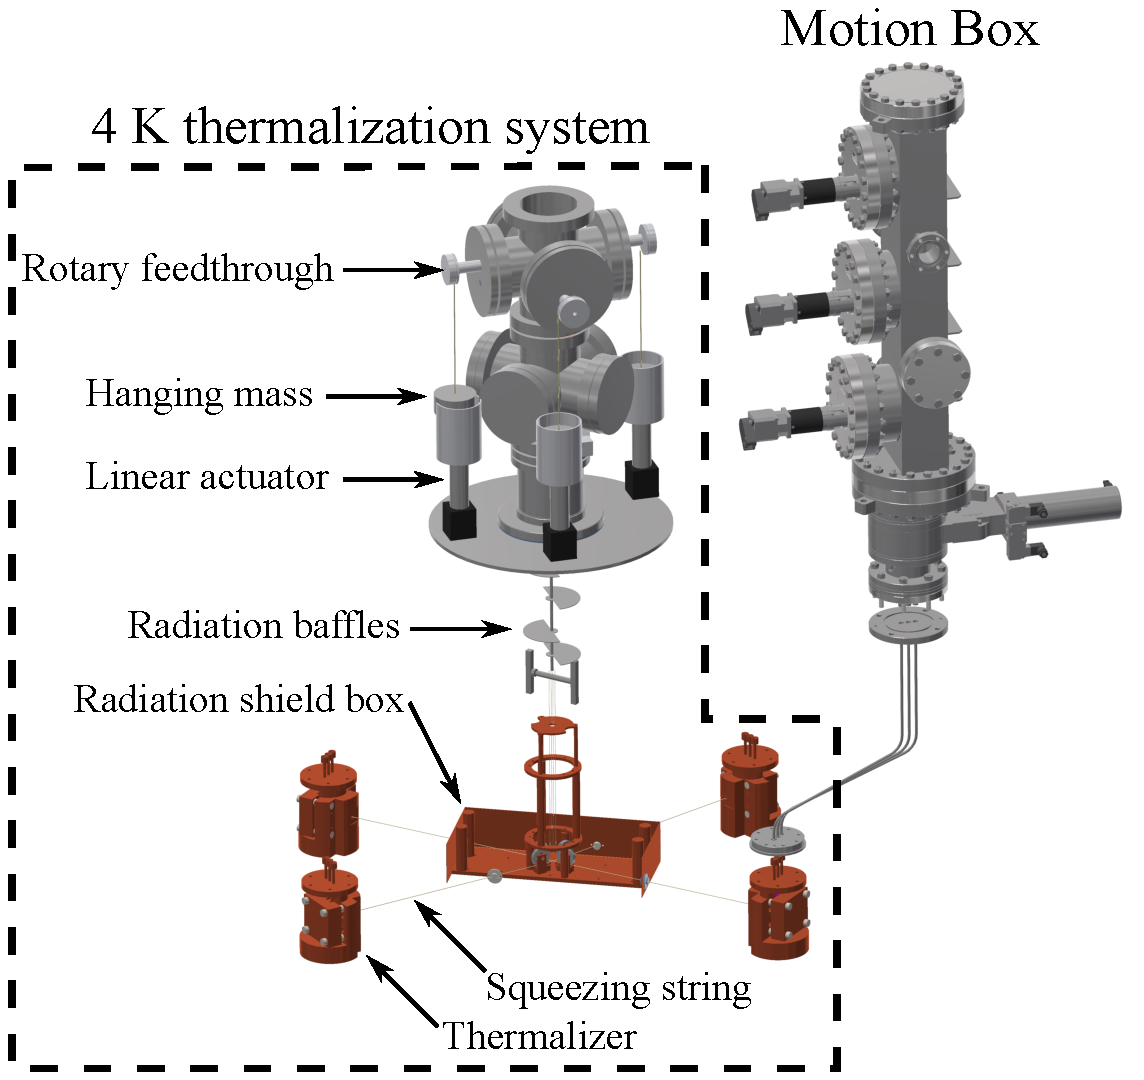
\includegraphics[width=\textwidth]{Figures/thermalization_system_labeled.pdf}
\caption{}
\label{fig:4K_thermalizer_system}
\end{subfigure}
\qquad
\begin{subfigure}[t]{0.44\textwidth}
\centering
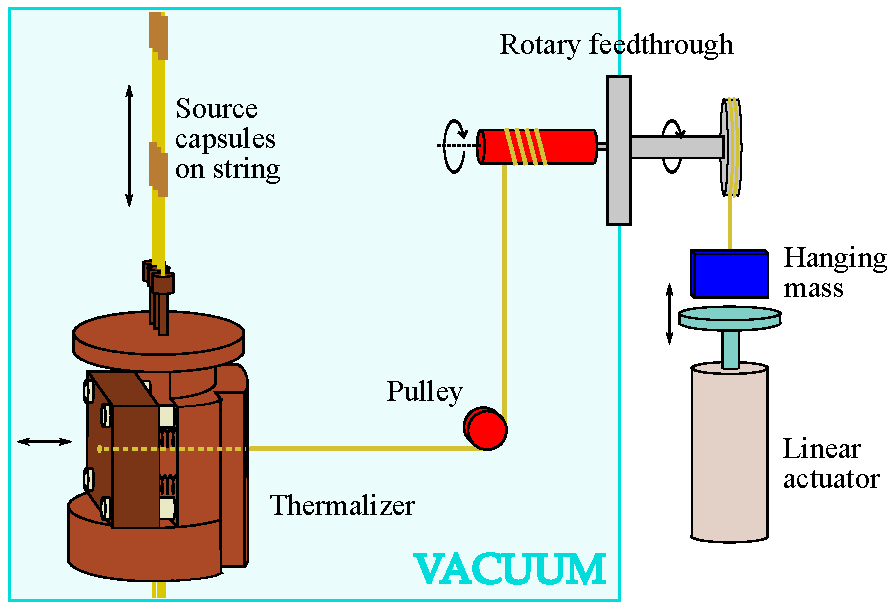
\includegraphics[width=\textwidth]{Figures/Thermalizer_schematic_labeled.pdf}
\caption{}
\label{fig:4K_thermalizer_schematic}
\end{subfigure}
\caption[The 4-K thermalization setup for the DCS]
{The 4-K thermalization setup for the DCS.
In (a), the setup for the system in conjunction with a motion box is shown (not shown are the other 3 motion boxes).
In (b), the mechanism for activating the thermalizers is shown.
A kevlar string connects the moving copper block through a pulley connected to the rotary feedthrough and a hanging mass that can be held up by a linear actuator.
In this way, moving the linear actuator up and down releases and activates the thermalizer, respectively.
Not shown is a metal ring that separates the kevlar string coming out of the shield box from the kevlar string from the thermalizer which reduces the thermal load and mechanical stress on the Kevlar.
Figure from \cite{Cushman:2016cnv}.}
\label{fig:DCS_4K_schematic}
\end{figure}

These thermalizers consist of a moving copper block and a copper base, with the copper block pushed away by a spring.
The copper block is activated by another Kevlar string that, when pulled, pushes the copper block onto the copper base.
The cooling time decreases as the force between the copper block and capsule increases until it reaches a maximum, and thus a force of 32 N was chosen as the force to apply as it would not damage the capsules.
This force is applied by a mass hanging from a pulley over a linear actuator. When the linear actuator pushes up on the mass, the thermalizer is opened, while, when the linear actuator moves down, the weight of the hanging mass applies the 32 N of force to the capsule.
The reason that the cooling is performed at the 4-K stage is that the cryostat still retains significant cooling power, as shown in \autoref{tab:cryostat_cooling_power}, yet can still cool the capsules to low enough temperatures.
Most of the cooling of the capsules is done at this position and this thermalization process over an entire string is a significant fraction of its total deployment time.
The size of the thermalizers is such that two source capsules can be inside the thermalizer at a time, and, similarly, up to four of the closer-packed weight capsules.

In order to determine the effectiveness of the cooling applied by the thermalizers, each thermalizer is instrumented with a thermometer\footnote{Although, due to a design flaw in the electronic circuit which inputs power to the block when open, this can be difficult to determine from the 4-K thermalizer thermometers alone.} on the copper block.
In addition, to verify that the thermalization of the thermalizers was sufficient, thermometers were also added to the 600-mK tubes, at varying locations as shown in \autoref{fig:600mK_thermometers}, to verify the thermalization of each capsule.
The thermometer used on each of the thermalizers is a CX-1010-SD Cernox\footnote{\RaggedRight\url{https://lakeshore.com/Pages/PackagesCX.aspx.}} thermometer calibrated to 1.4 K, and mounted at varying locations on each of the 600-mK guide tubes are CX-1030-SD Cernox thermometers, with 10 calibrated to 1.2 K, and the other 2 calibrated to 300 mK.
During Run 3, one of the cold commissioning runs of the cryostat and the DCS, the 10 thermometers on the 600-mK guide tubes calibrated at 1.4 K were then calibrated down to below 600 mK.

\begin{figure}[htbp]
\centering
\begin{subfigure}[t]{0.9\textwidth}
\centering
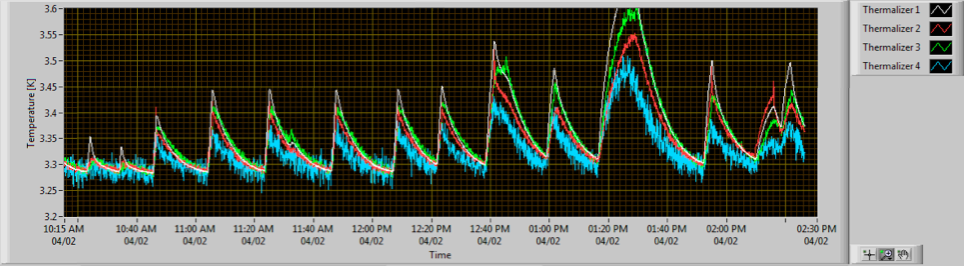
\includegraphics[width=\textwidth]{Figures/Thermalizer_operation.png}
\caption{}
\label{fig:4K_operation}
\end{subfigure}
\qquad
\begin{subfigure}[t]{0.9\textwidth}
\centering
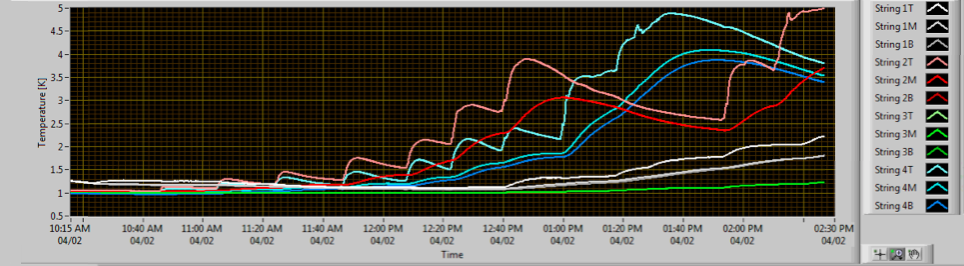
\includegraphics[width=\textwidth]{Figures/Chicane_operation.png}
\caption{}
\label{fig:Chicane_operation}
\end{subfigure}
\caption[The thermometers on the 4-K thermalizers (a) and the 600-mK tubes (b) during a deployment]
{The thermometers on the 4-K thermalizers (a) and the 600-mK tubes (b) during deployment.
Here, the 4 thermalizers simultaneously squeeze on capsules in regular intervals, with the openings of the thermalizers corresponding with the peaks in (a).
When the capsules reach the 600-mK guide tubes, the capsules begin to release heat into the tubes, which causes the tubes to warm up as seen in (b).
Due to the higher capsules on the string being warmer than the bottom capsules, the 600-mK guide tubes are heated more from later capsules, despite more of the mass of the string in the weight capsules.
The thermometers that are located on the inner guide tubes with a chicane observe a much larger rise in temperature than the outer guide tubes as more heat is extracted inside the chicane.
Not all 12 600-mK thermometers survived the cooldowns and installation, but enough are on each set of guide tubes to be able to measure the temperature of the incoming capsules.}
\label{fig:Thermalization_operation}
\end{figure}

\begin{figure}[htbp]
    \centering
    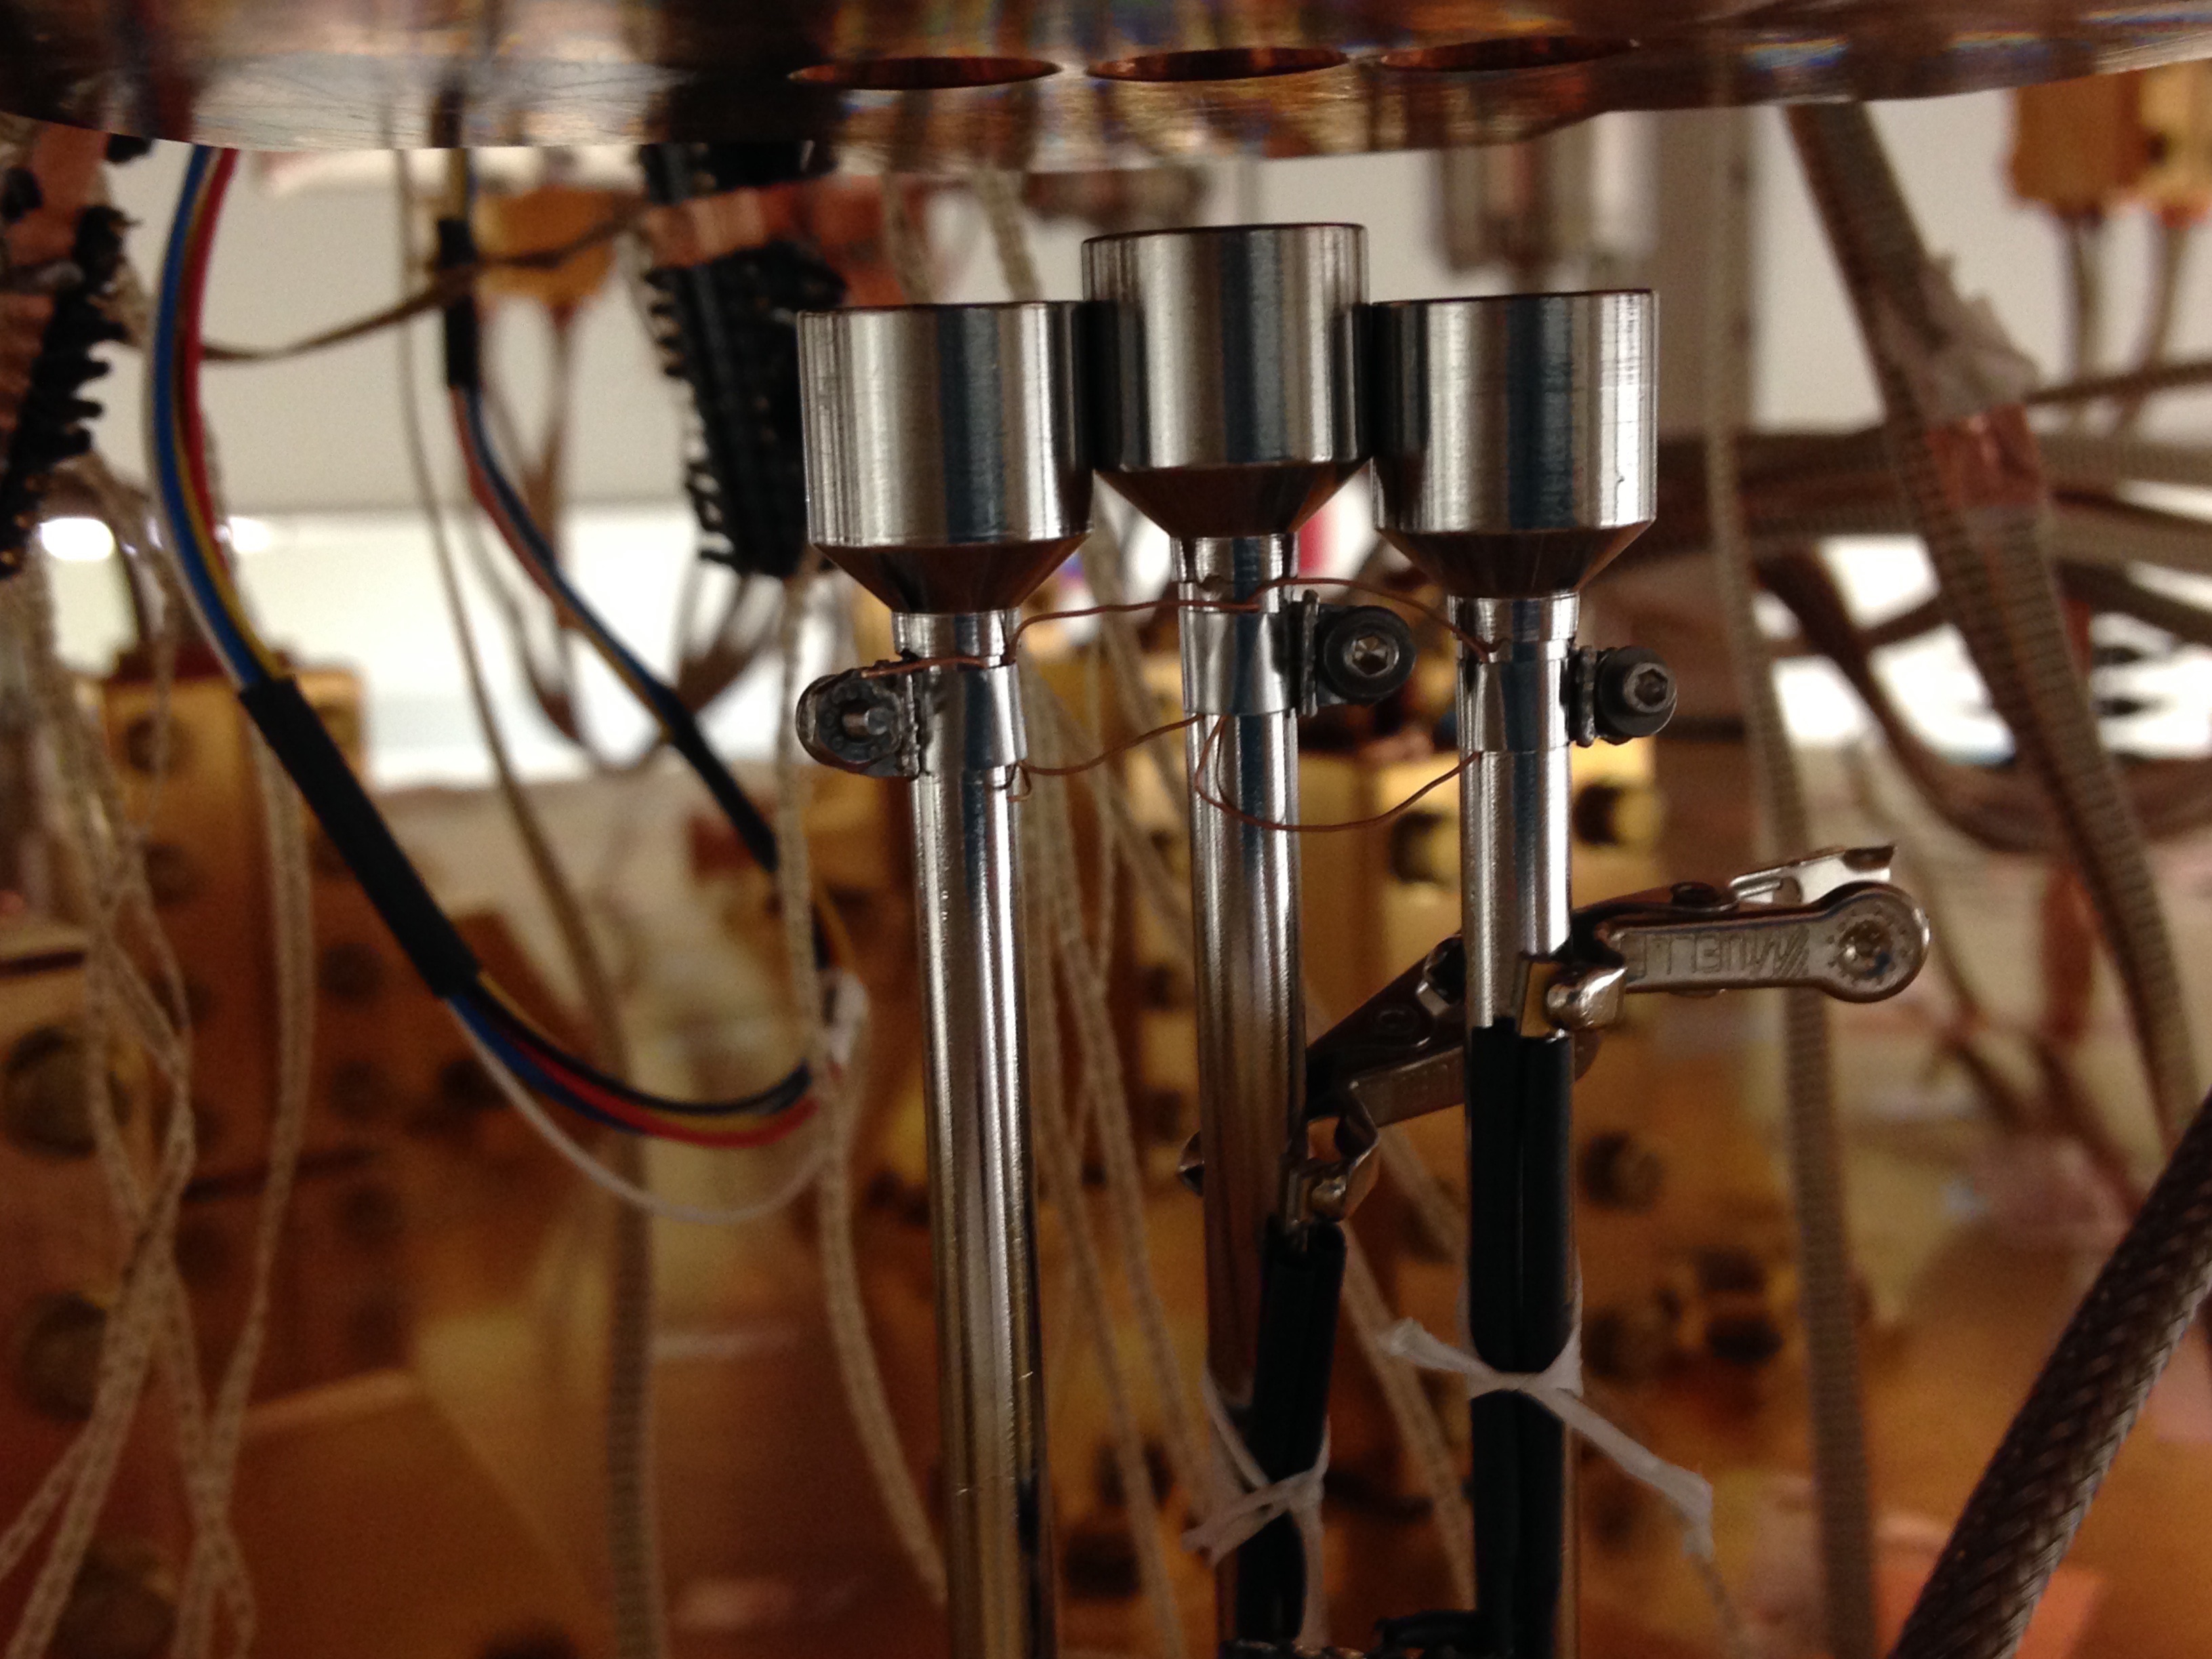
\includegraphics[width=0.8\linewidth]{Figures/ChicaneThermometers.JPG}
    \caption[The 600-mK guide tube thermometers]
{The 600-mK guide tube thermometers.
These thermometers are used to determine the temperature of the capsules as they leave the 4~K thermalizer into the 600~mK guide tubes.
2 of the 3 thermometers are shown here and are held and thermalized to the tube with modified alligator clips.
Note the small copper wire that was connected to each of the guide tubes.
This wire connects each of the guide tubes such that the thermometers from one guide tube can measure the temperature rise on another guide tube which is particularly useful for tubes with a faulty thermometer connection.}
    \label{fig:600mK_thermometers}
\end{figure}


\subsection*{Software Control of the DCS}
\label{ssec:Software Control of the DCS}
As mentioned in \autoref{sec:DCS_Overview}, the DCS needs to be operated and handled in a controlled and stable fashion, and, to this end, the choice was made to operate the entire system through software-controlled motors.
A computer running Labview\footnote{\RaggedRight\url{http://www.ni.com/en-us/shop/labview/labview-details.html}} controls and monitors the hardware components of the DCS including the motors, the load cells, thermometers, pressure sensors, and other components described previously.
These systems are described in detail in \cite{JeremyThesis}, but in this section, I will describe the interlocks used to ensure the safety of the system with even more details in \autoref{ch:DCS Guide and Manual}.
One of the first to mention are the interlocks for the vacuum systems.
As remote operation is possible through the software control, a person on-site needs to be available to activate the gate valves below the motion boxes that connect to the IVC.
This prevents any accidental openings of the motion box to the IVC, which has the potential to be a catastrophic event.
The other interlocks relate to the motion and tension on the string itself.
As mentioned above, the home switch and global stop switch are two-state switches that are used to stop motion when they are triggered.
However, the load cell allows for more complex interlocks on the system as the tension in the string is measured constantly during their motion.
This information is used to create a ``load cell profile" that is an averaging of multiple deployments of the string through the guide tubes.
As the particular geometry of the guide tubes affects the tension of the strings, e.g. a vertical section has tension equal to the hanging weight of the source string, whereas an angled section has capsules slightly resting on the tubes, which decreases the tension in the string.
With this information, this allows the software to detect situations such as when the string has missed a funnel and is beginning to rest on the cryostat or if there is an obstruction in the cryostat such as ice as shown in \autoref{fig:load_cell_profile}.
In addition, the software uses the load cell to determine and stop motion in case of sudden changes in the tension.
Because the length of the string that contains the weight capsules is a few cm long, this quick step in the voltage is another indication of the string stopping. 
It also allows for an independent verification of the string position inside the cryostat in addition to the position readings from the encoder.
With these checks, the dangerous scenarios that can be caused when a string fails to deploy properly, which can cause the string to misspool on the drive spool shaft, or to form a knot, each of which would be problematic for continued DCS performance or detector operation.

\begin{figure}
    \centering
    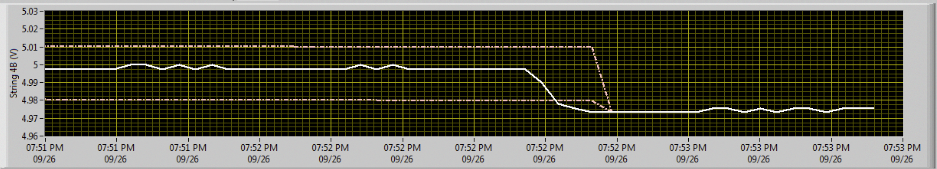
\includegraphics[width=0.8\linewidth]{Figures/LoadCellProfile.png}
    \caption[The load cell readings and profile during a string deployment]
    {The load cell readings (white) and profile (red) during a string deployment.
    The load cell profile is an averaged reading from past deployments and contains a band of acceptable values inside.
    When the load cell is outside of the accepted values for long enough, an error is returned, as was the case here.}
    \label{fig:load_cell_profile}
\end{figure}

\subsection*{Impact on Cryostat}
One of the main effects on the cryostat from the DCS in operation is the thermal stress it applies to the system.
Were the DCS to drop the strings into the cryostat, the deployment would take only a matter of seconds, but this would catastrophically affect the operation of the dilution refrigerator.
This constraint is the main constraint on the deployment speed and is one of the main constraints on the extraction speed.
The effect of the source strings is negligible down to the 4-K stage, but even the radiative heat load of the strings as they reach the 4-K thermalizers applies a heat load to the 600-mK plate, as shown in \autoref{fig:600_mk_Precool}.
\begin{figure}
    \centering
    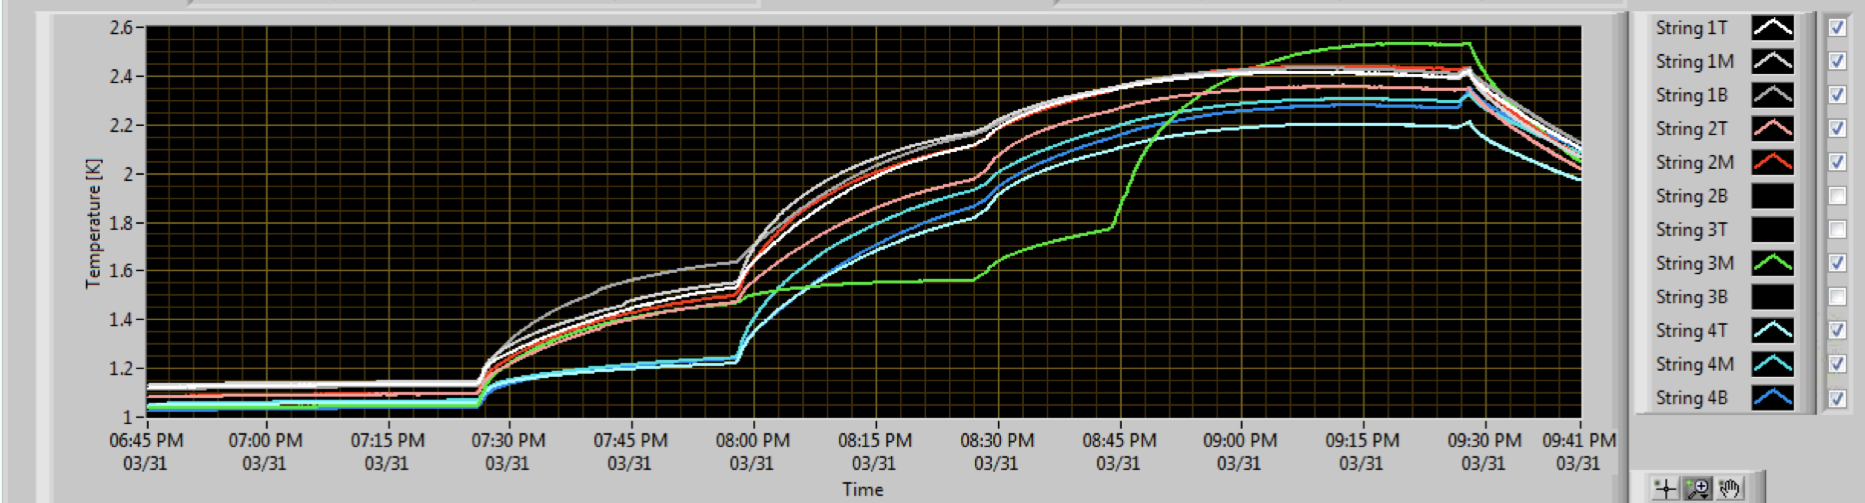
\includegraphics[width=0.8\linewidth]{Figures/600mK_temperature_during_precool.png}
    \caption[The temperature of the 600-mK thermometers as the source strings reach the 4-K stage]
    {The temperature of the 600-mK thermometers as the source strings reach the 4-K stage.
    The heat load increases as more strings are successively deployed until the 4-K thermalizers are closed, cutting off the line-of-sight between the 600-mK stage and the capsules in the s-tubes above.}
    \label{fig:600_mk_Precool}
\end{figure}
To reduce the temperature of these capsules before reaching the 600-mK stage, a two-stage process is undertaken.
First, the strings are deployed to just above the 4-K stage at a speed of 75 mm/min\footnote{The motors can operate the strings at speeds up to 500 mm/min and as low as 1-2 mm/min.
As the duration of the deployment in this region above 4-K is not a significant amount of time given the entire time for deployment, a higher speed is not used here.}.
Then, after waiting $\sim12$ hours for pre-cooling, the strings begin a set of squeezes in the thermalizer.
These squeezes vary in length from 10-minute squeezes on the lowest capsules that have cooled the most during the pre-cooling to 20-minute squeezes on the capsules that are the highest on the string.
In fact, due to the geometry of the cryostat and the fact that the active region of the string is larger than the distance between cryostat stages, the top of the capsules are less than 20 cm below the proximity sensor during the first thermalizer squeezes, which is the reason why longer squeezes become necessary.
After the thermalizer squeezes on the strings, the string is lowered slightly below the end of the thermalizer to allow for another string to be thermalized and for more time for cooling of the capsules to temperatures below 4 K.
During this time, the speed that the strings move is also decreased, in order to reduce the thermal ``shock" of deploying the relatively warm capsules to increasingly colder regions.
In addition, this slower speed increases the time to respond in case the capsules are warmer than anticipated and begin warming the cryostat.
As the string are lowered into the 50-mK and 10-mK stages of the cryostat, the outer strings impact the cryostat to a lesser degree than the inner strings, as the 50-mK stage can handle more heat before cooling at the 10-mK stage is impacted, as shown in \autoref{fig:50mK_vessel_heating}.
\begin{figure}
    \centering
    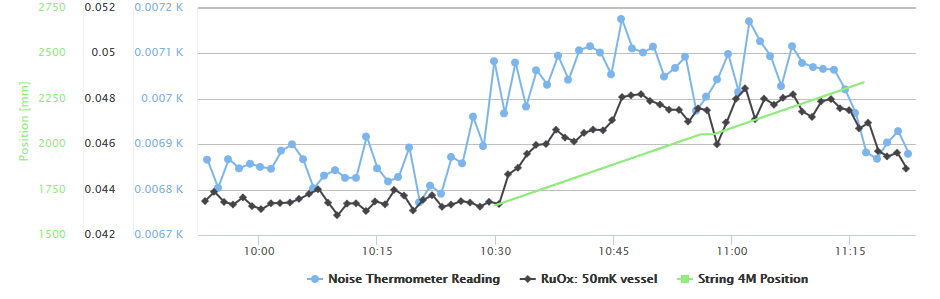
\includegraphics[width=0.8\linewidth]{Figures/OuterStringHeating.png}
    \caption[The heating of the 50-mK vessel during an outer string deployment]
    {The heating of the 50-mK vessel during an outer string deployment.
    As the string, in green, moves into the detector region, the 50-mK vessel warms by 6 mK, while the thermometer at the 10-mK stage, the noise thermometer, warms by 0.3 mK.
    This data comes from a test run before the installation of the detectors, as the thermometers on the vessels are disconnected during later operations.}
    \label{fig:50mK_vessel_heating}
\end{figure}
The largest effects on the detectors come from the inner strings as they are deployed into the 10-mk region.
These effects are due to both the warm capsules entering the region, and due to the friction of the capsules moving against the guide tubes.
In early tests in the 10-mK region before the detector region guide tubes were installed, the heating would be only a few mK.
However, with the detectors installed, lowering the available cooling in the region, and the guide tubes also installed, increasing the vibrational and frictional effects of the deployment, the impact on the cryostat increased significantly.
During these later deployments, the temperature of the cryostat reached approximately 25 mK while the strings were being lowered into this region.
When extracting the strings, the main constraints are due to the friction of the capsules as they move against the guide tubes.
In extraction, in contrast to deployment, the capsules are colder than the stages they pass through, but limiting the speed is the need to reduce the effect of this friction.
This friction is maximized at points where there is a bend in the guide tubes, such as the bend at the 10-mK plate for the inner source strings.
The heating in this case depends strongly on the speed with which the strings are extracted, and the choice was made to keep the impact on the base temperature of the cryostat to similar levels as 25 mK that is reached during deployment.
As the source strings leave the 50-mK region, this issue no longer becomes significant and the speed of the calibration sources can be increased as the strings pass through more cryostat stages\footnote{However, there is still an effective ``speed limit" as an obstruction that the string encounters on the way up through the cryostat could trigger the emergency stop switch if the strings are moving too quickly.}.

\section{Calibration Simulation}
In order to properly understand the activities of the sources and the optimal duration for calibrations of the detectors, Monte Carlo simulations of the calibration sources are performed.
These way in which these simulations are performed is described in more detail in \autoref{ch:Simulation in CUORE}, but the results of these simulations for calibration are described here.
As the role of calibration is to define the energy scaling of the detector response, viz. how to map the output voltages of the NTD thermistors to the amount of energy deposited into the crystal, the use of a ``standard candle" is needed in calibration.
The well-understood decay chain of $^{232}$Th serves this purpose as the calibration sources used in the DCS, as it produces multiple monoenergetic photons ranging from the 239 keV from $^{212}$Pb to the 2615 keV from $^{208}$Tl shown in \autoref{fig:Outer_and_inner_spectra}.
\begin{figure}[htbp]
    \centering
    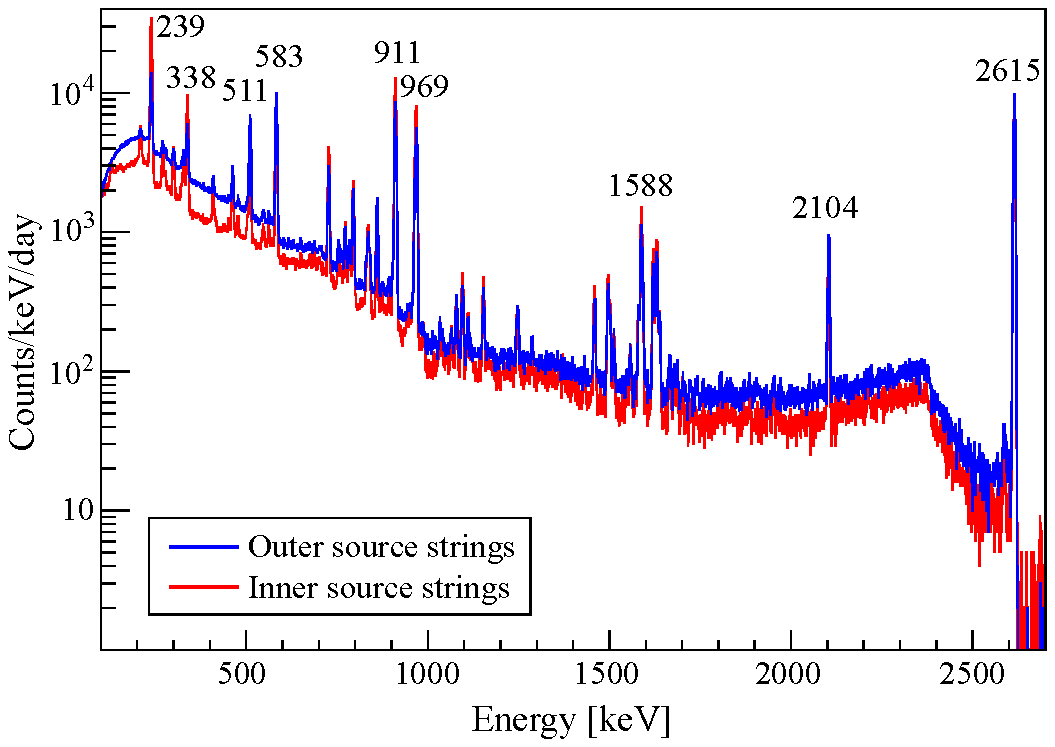
\includegraphics[width=0.9\linewidth]{Figures/overlapping_spectra.pdf}
    \caption[The energy spectra from the inner and outer calibration sources]
    {The energy spectra from the inner and outer calibration sources.
    The outer sources have lower relative peak heights as photons emitted need to also pass through the 50-mK and 10-mK shields, which can be seen especially at the 239 keV peak. 
    While there are multiple visible peaks in the spectra, the six peaks at 239, 338, 583, 911, 969, and 2615 keV are used for calibration.
    The peaks are caused by the de-excitation of $^{212}$Pb, $^{228}$Ac, $^{208}$Tl, $^{228}$Ac, $^{228}$Ac, and $^{208}$Tl nuclei, respectively.
    Figure from \cite{Cushman:2016cnv}.}
    \label{fig:Outer_and_inner_spectra}
\end{figure}
As the important factors to consider in calibration of the detectors, the calibration sources need to be optimized to irradiate the towers with equal rates for all the detectors.
The rates at which the detectors see events are shown in \autoref{fig:Channel_Event_Rates} and \autoref{fig:Peak_event_rates}.
\begin{figure}
    \centering
    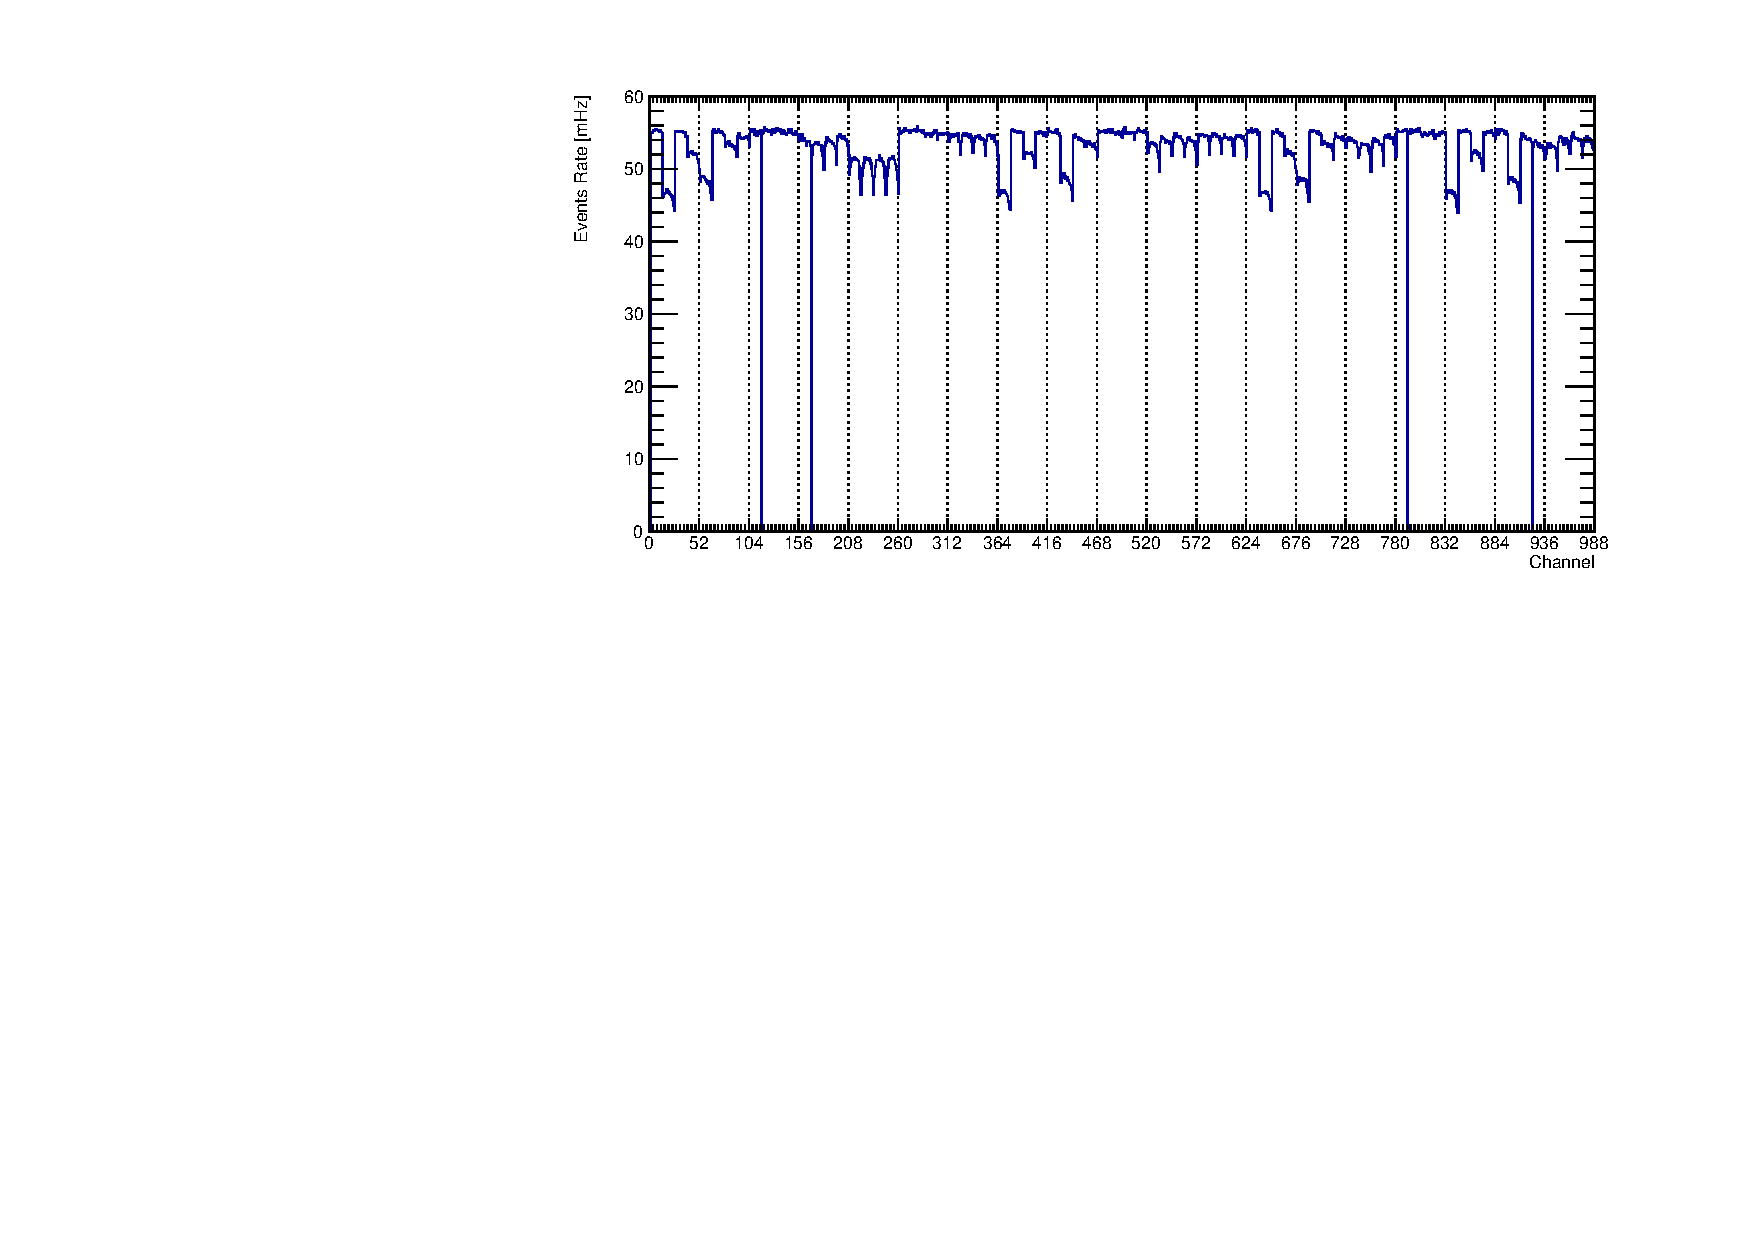
\includegraphics[width=0.9\linewidth]{Figures/ChannelEventRates.pdf}
    \caption[The rates on each crystal due to the calibration source after pileup cuts]
    {The rates on each crystal due to the calibration source after pileup cuts.
    The rates are nearly consistent across all the channels, as at higher rates, pileup becomes a limiting factor on the measured rates.
    Note that the 4 channels without counts are the dead channels in CUORE where the NTD connection failed.}
    \label{fig:Channel_Event_Rates}
\end{figure}
\begin{figure}
    \centering
    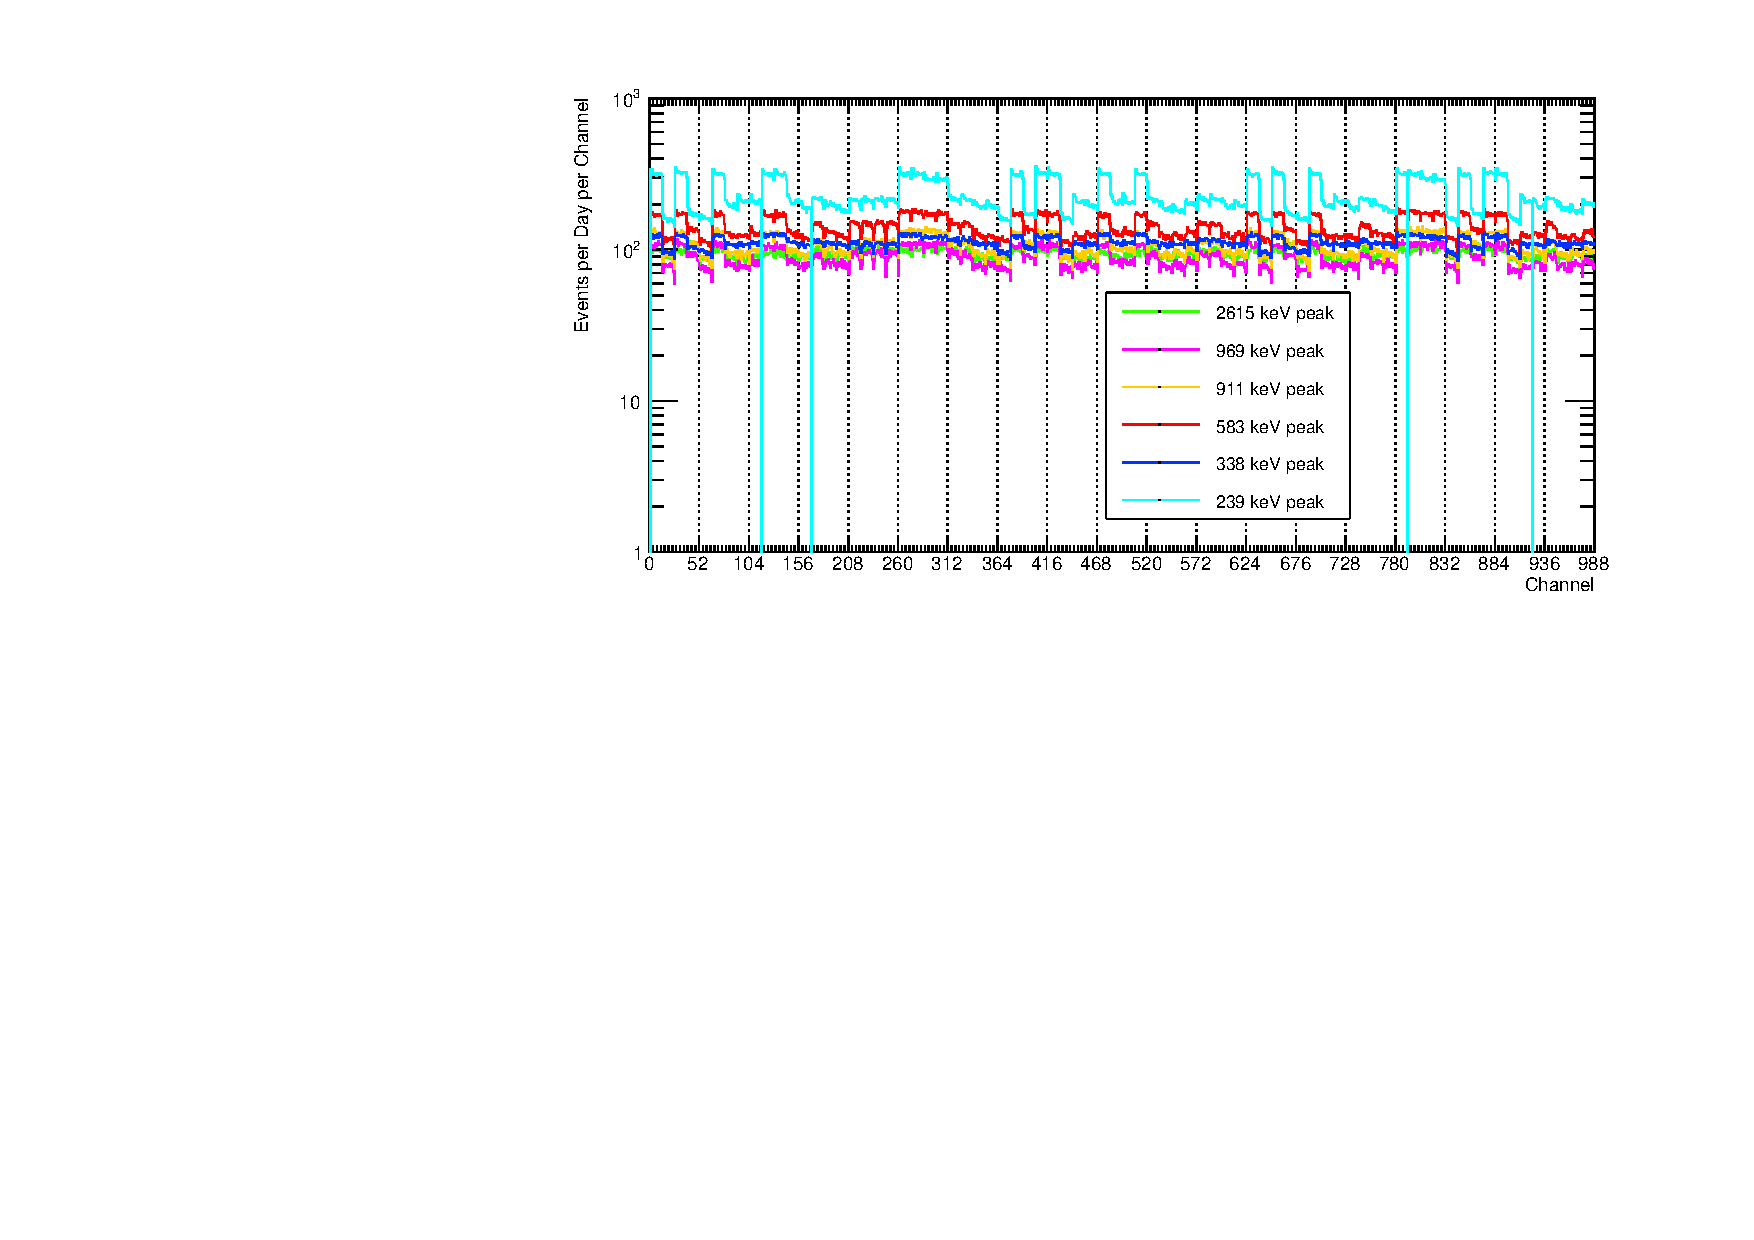
\includegraphics[width=0.9\linewidth]{Figures/PeakEventRates.pdf}
    \caption[The rates of each peak used in calibration]
    {The rates of each peak used in calibration.
    The lower-energy peaks have a stronger channel dependence than the higher-energy peaks, due to the towers self-shielding crystals without a direct line-of-sight to a calibration source.}
    \label{fig:Peak_event_rates}
\end{figure}
This nearly uniform distribution is achieved by the interplay of the inner and outer sources and by boosting the activities of the lowest and highest capsules as shown in \autoref{tab:calibration_activities}.
The effects of this boosting for each string is shown in \autoref{fig:calibration_source_contributions}.
\begin{figure}[htbp]
\centering
\begin{subfigure}[t]{0.9\textwidth}
\centering
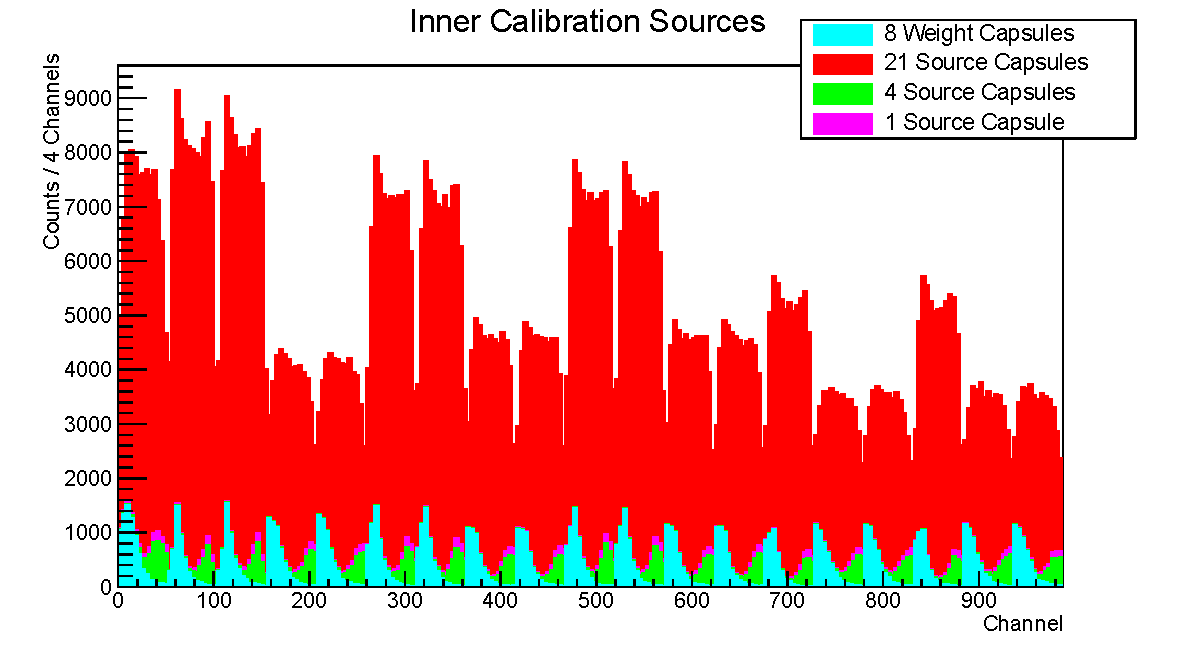
\includegraphics[width=\textwidth]{Figures/InnerCalibrationSources.pdf}
\caption{}
\label{fig:inner_calibration_sources}
\end{subfigure}
\qquad
\begin{subfigure}[t]{0.9\textwidth}
\centering
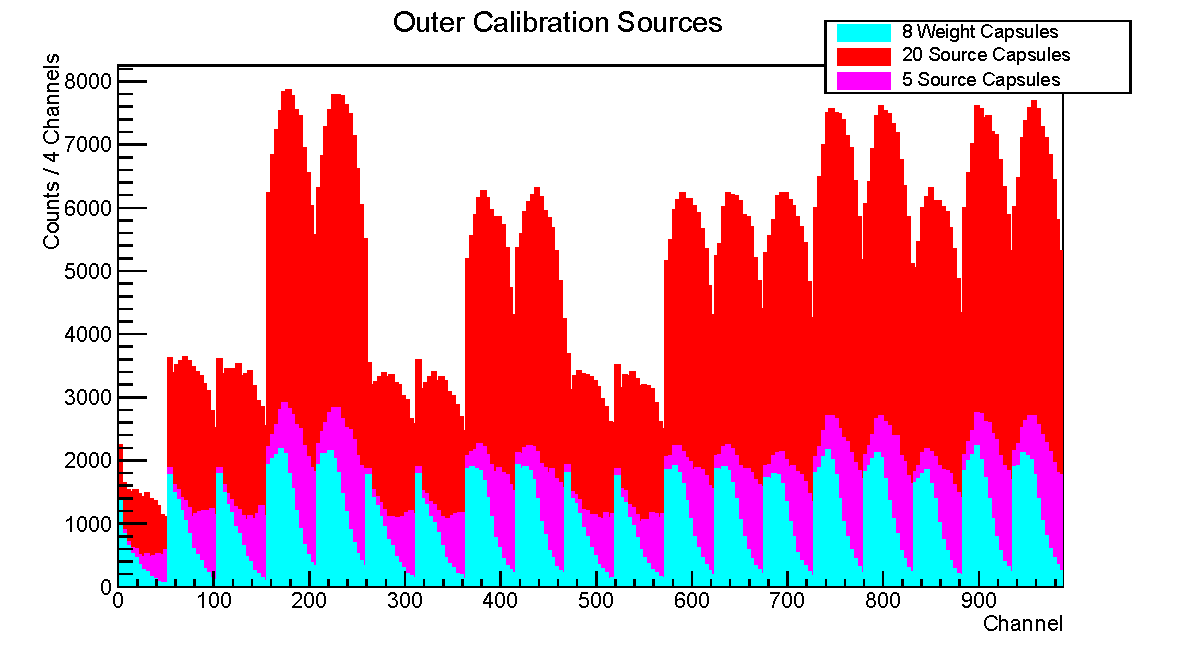
\includegraphics[width=\textwidth]{Figures/OuterCalibrationSources.pdf}
\caption{}
\label{fig:outer_calibration_sources}
\end{subfigure}
\caption[Stacked histograms showing the contributions to the counts from each set of capsules on the inner (a) and outer (b) strings]
{Stacked histograms showing the contributions to the counts from each set of capsules on the inner (a) and outer (b) strings.
The y-axis is arbitrary and the channels are binned according to each floor on each tower.
The boosted activities of the top and bottom capsules, for reference see \autoref{tab:calibration_activities}, serve to keep the rates as uniform as possible although the outer sources could have had more significant boosting.}
\label{fig:calibration_source_contributions}
\end{figure}
In addition, the uniform distribution comes from the pileup cuts implemented in CUORE.
These cuts are described in more detail in \autoref{ch:Data Acquisition and Processing}, but their effect is most strongly felt for the calibration data, as calibrations are the time when the detectors observe significantly higher rates than the $\mathcal{O}(1)$ mHz during physics runs.
This effect on the calibration rates is shown in \autoref{fig:pileup_effects}.
\begin{figure}
    \centering
    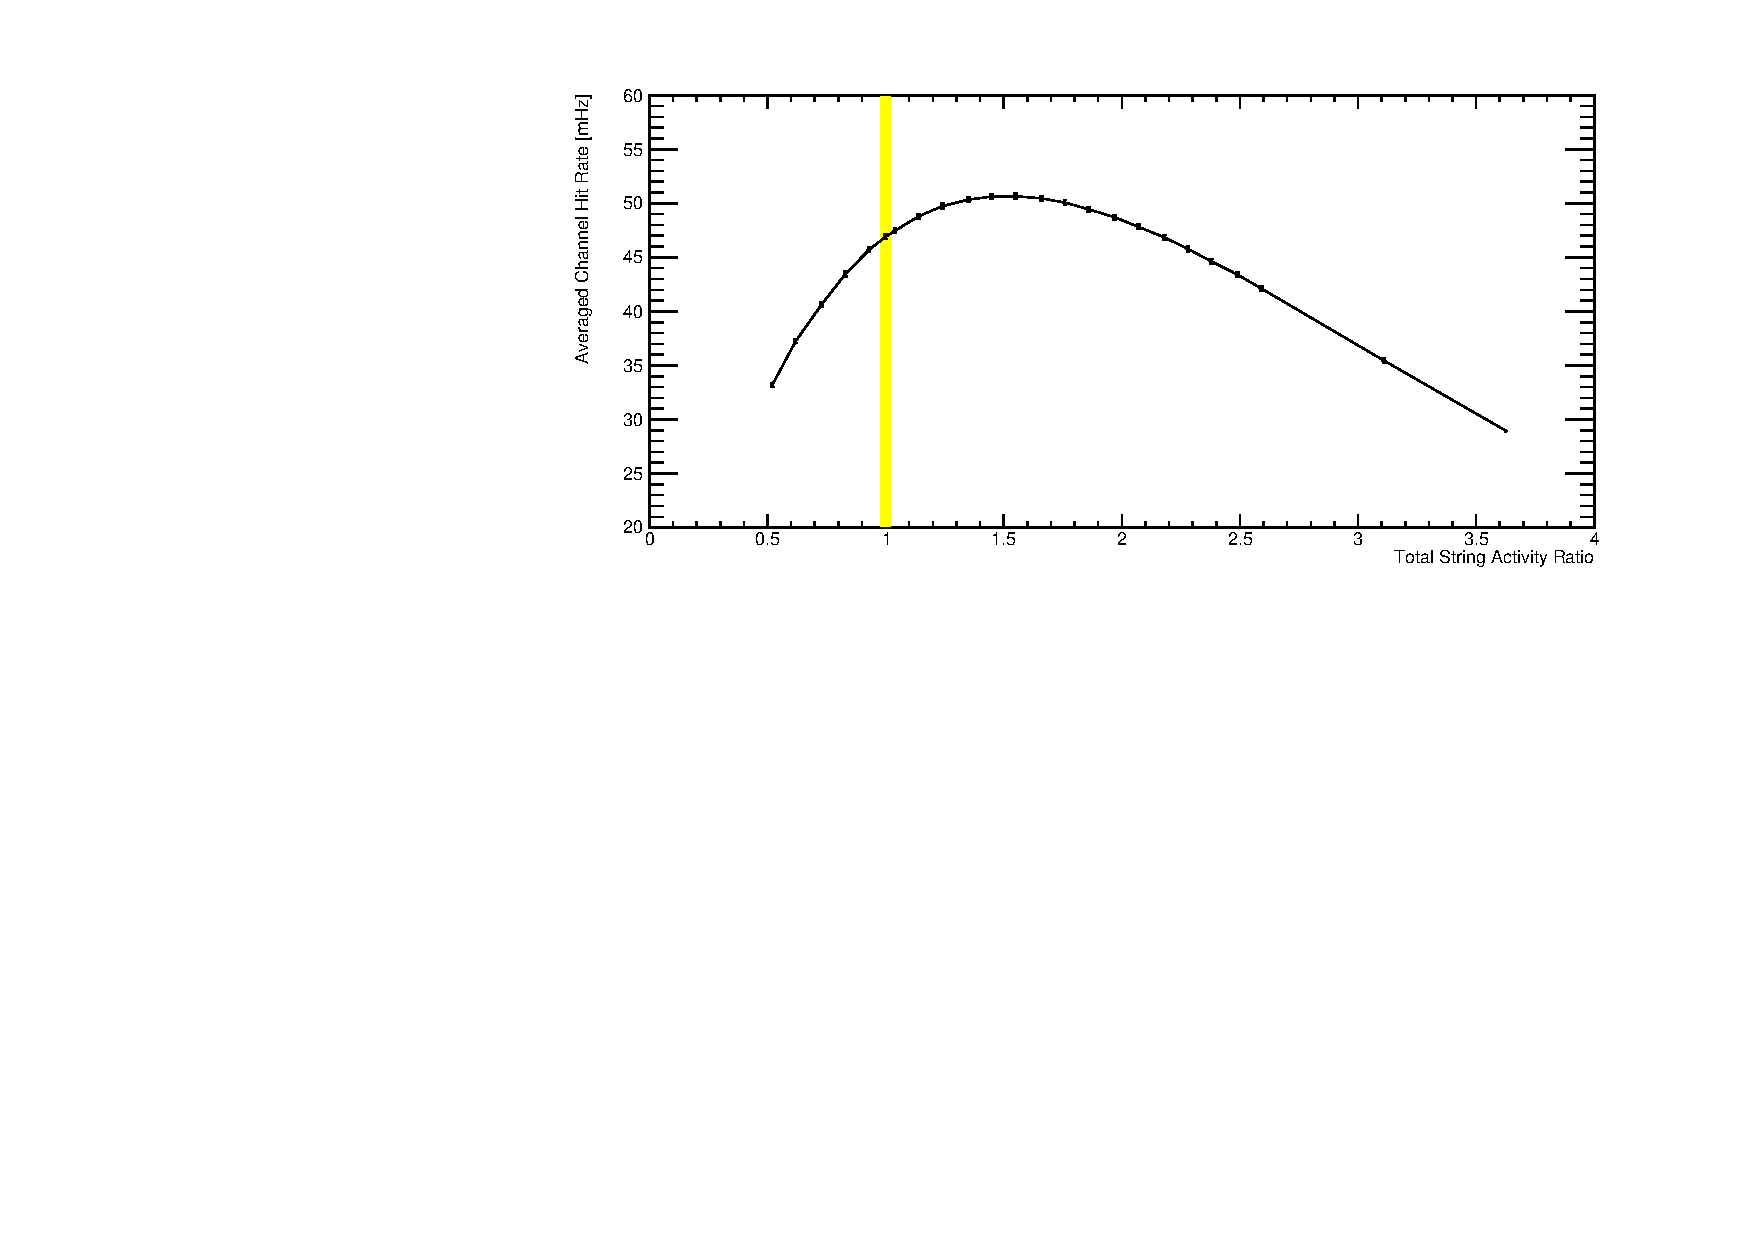
\includegraphics[width=0.9\linewidth]{Figures/HitRate_Activity.pdf}
    \caption[The averaged rate over all the detectors for various scaled activities of the source strings]
    {The averaged rate over all the detectors for various scaled activities of the source strings.
    The rate for the actual sources is highlighted in yellow.
    This plot was developed for the original pileup window of 7.1 s (3.1 s before, 4.0 s after) between events, but this was changed to 10 s (5 s before, 5 s after) between events which has the effect of pushing the curve to the left and decreasing the maximum rate.}
    \label{fig:pileup_effects}
\end{figure}

The most important peak in the calibrations is the 2615 keV $^{208}$Tl peak due to its proximity to the 2528 keV Q-value of \zeronubb~in ${130}$Te and it being significantly higher than the other peaks used in the calibration.
Thus, the rate of this peak drives much of the time used for calibration.
Again, considering that the purpose of the calibration is to determine the mapping between the output voltages and the energy deposited into the crystals, enough counts need to be collected of each peak to provide the proper mapping.
As these fits are generally Gaussian in nature, $\sim50$ counts from a particular peak is generally enough to calibrate a detector, and the time it takes to reach 50 counts is shown in \autoref{fig:FullString_50counts}.
\begin{figure}
    \centering
    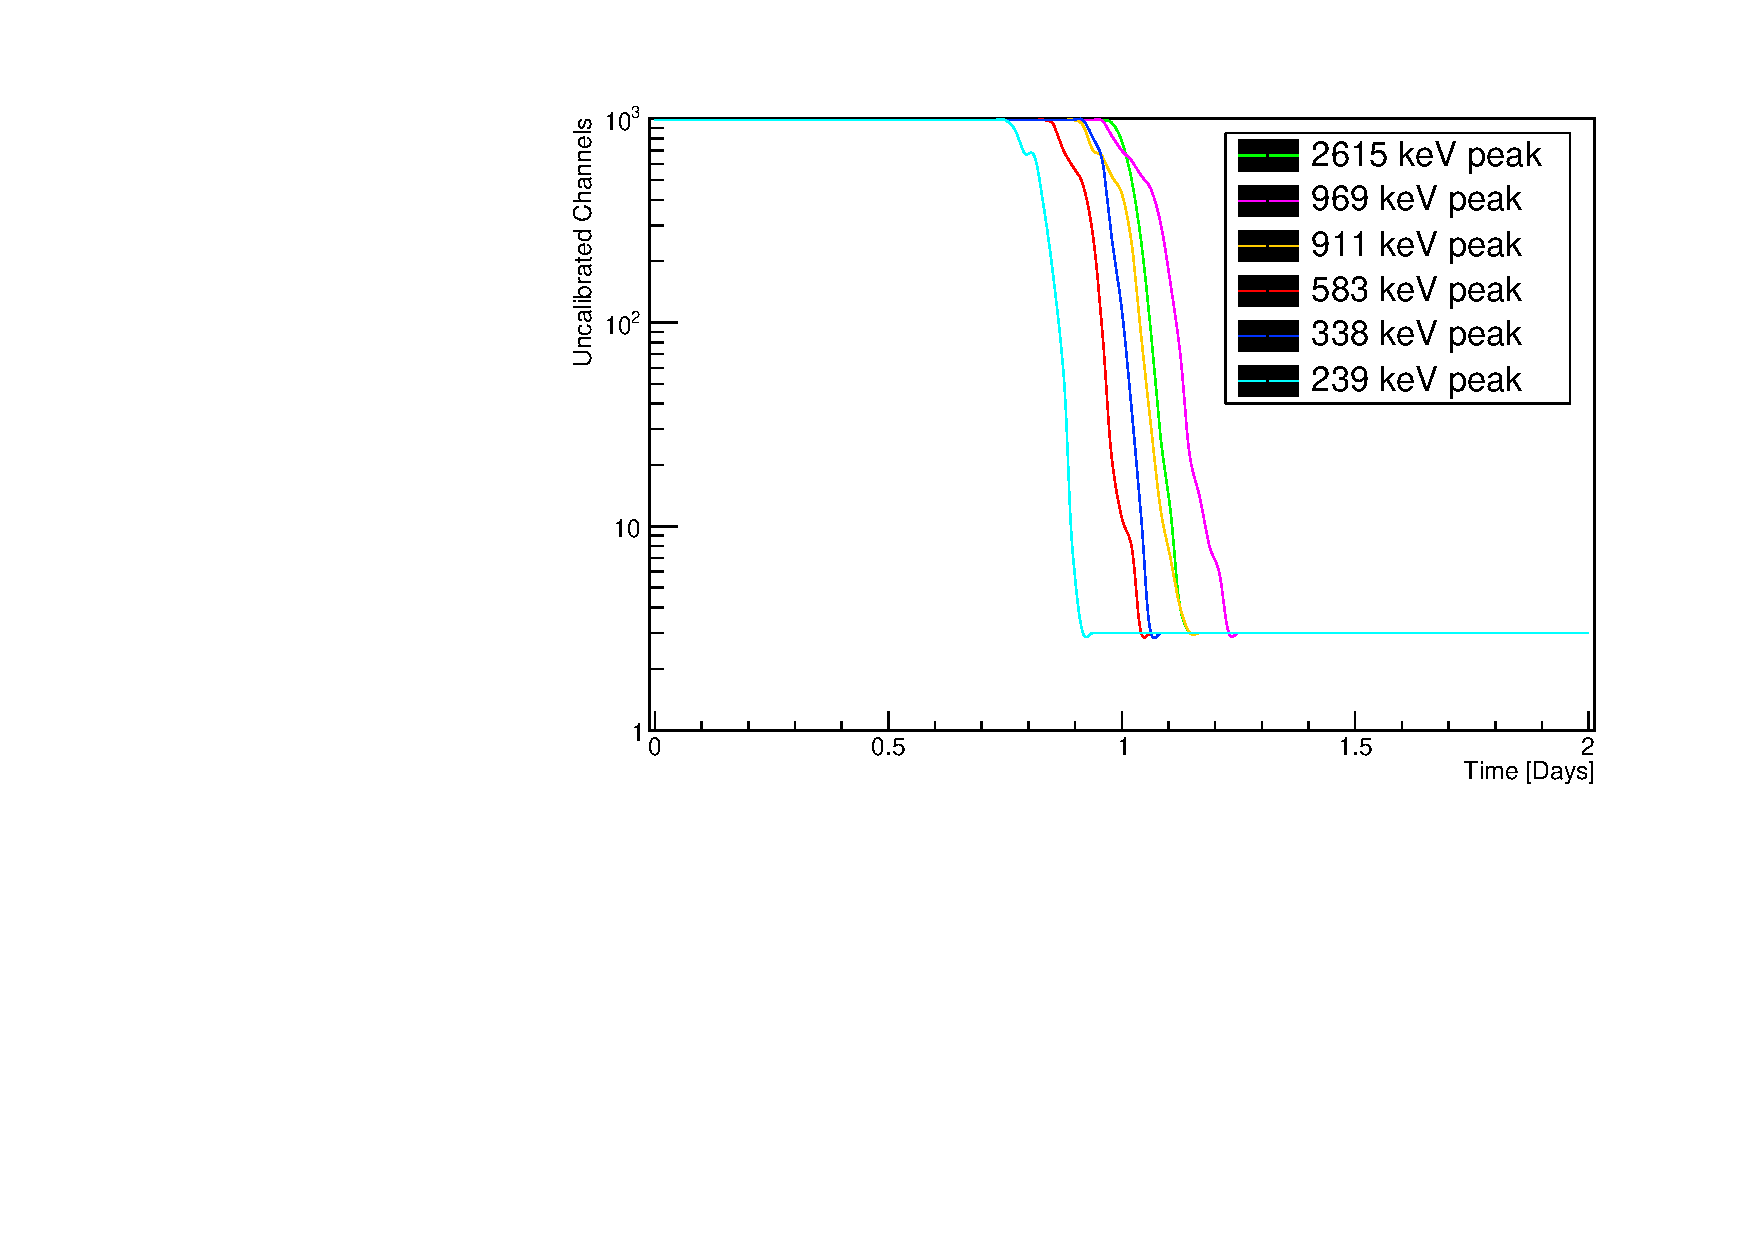
\includegraphics[width=0.9\linewidth]{Figures/FullString_50Counts.pdf}
    \caption[The time it takes to reach 50 counts for each peak during a calibration]
    {The time it takes to reach 50 counts for each peak during a calibration.
    It requires approximately one day for each of the peaks to reach 50 events, and all of the channels are calibrated at roughly the same time.}
    \label{fig:FullString_50counts}
\end{figure}

\section{Calibration Performance}

\subsection*{Calibration Strategies}
\label{ssec:Calibration Strategies}

When deploying strings, it would be considerably simpler if one could deploy all the strings simultaneously down into the cryostat; however, there are multiple considerations that need to be taken into account during the operation.
Firstly, one of the main constraints is that no strings from the same motion box can pass through a 4-K thermalizer while it is squeezing on another string.
As the time it takes to squeeze on each set of capsules takes 10-20 minutes, this process takes hours for each string, and requires cleverly arranging the schedule to reduce the overall time.
Secondly, the heat load from the calibration sources themselves is important.
The 4-K thermalization cools these capsules down, but the heat loads from both the friction and the still relatively warm capsules heats up each cryostat stage.
Therefore, only one inner source string is deployed into the detector region at a time, and up to two outer strings can be deployed outside the 50-mK vessel in parallel.
Since this procedure takes hours to complete, this is done in two stages.
First, there is a precooling stage, where the 12 calibration source strings are deployed into the cryostat from the motion boxes to a position where the weight capsules of each string are midway through the thermalizer.
Then, the thermalizer is closed on the string overnight, enabling the strings to cool down through contact with the walls of the s-tubes.
The second stage of deployment begins after the precooling stage completes. Then, two of the strings from each motion box are moved back out of the thermalizer, while the string that has been in the thermalizer begins its thermalization steps.
After the thermalizer has squeezed on each of the capsules on a string in succession, the string is moved $\approx5$ cm downwards out of the thermalizer for the thermalization on the next string to commence.
Now, two strategies are used to deploy the strings from the thermalizers.
In one strategy, strings are be deployed into the detector region while the 4-K thermalization steps continue, and, in the other, the strings are deployed only after all the 4-K thermalization steps have been completed.
In the strategy where the thermalizers are active during detector region deployments, the time it takes to deploy is approximately 20 hours from the start of thermalization after precooling.
In the strategy where the thermalization is completed before deploying strings into the detector region, the time it takes to deploy is approximately 24 hours.

\subsection*{CUORE Calibrations}
\label{ssec:CUORE Calibrations}
Unfortunately, the DCS has not performed perfectly while the detectors have been in place.
The main cause of the issues is due to the fact that gas freezes in the s-tubes and blocks the motion of the capsules down into the cryostat.
This issue prevents the strings from deploying into the cryostat, and, in the worst cases, freezes over a string and prevents the weight capsules from extracting back into the motion boxes.
What exacerbates this issue is the small tolerances between the inner diameter of the s-tube (4.0 mm) and the width of the weight capsules including their teflon heatshrink ($\approx$3.2 mm).
This means that a deposit of ice with cross-sectional area as small as 18 mm$^2$ can completely stop the motion of the strings.
Assuming that the length of tube with ice is $10$ mm long, this means that a 180 mm$^3$ volume of ice is enough to prevent all the motion in a string.
This corresponds to a pressure of $\approx40$ mbar of water in a motion box at room temperature, or $\approx100$ mbar if all 3 s-tubes below the motion box are filled simultaneously.
Although the motion boxes are pumped while moving a string, they are only cryopumped through the s-tubes while calibration data is being collected with the strings deployed in the cryostat.
This cryopumping directly deposits the outgassed water from the walls of the motion box.
During short calibrations, this is not a significant problem, but this problem worsens over time as it requires the cryostat to warm up to properly remove the deposited gas\footnote{For nitrogen, this would require the s-tubes to warm above $\sim$70 K, but for water, would require the s-tubes to warm to nearly room temperature.}.
Initially, the cause of this was believed to be due to leaky gate valves under the motion box, but, as the problem persisted after the gate valves were replaced and warming the cryostat above 100 K did not remove the frozen gas, the problem appears to be due to water from the outgassing of the motion boxes.

In addition, another problem appears when the inner source strings reach the vertical detector region guide tubes.
For these strings, some of them are unable to fully deploy down through these tubes and behave as if there is increased friction between the capsules and the tubes that prevents their continued downwards motion.
This stops four of the inner source strings at different locations in the detector region guide tubes, and two of the six have been entirely unaffected by it.
This issue was never seen during test deployments with the cryostat at room temperature, and given its reproducibility, seems to be an issue with unexpectedly high friction along the guide tubes, either in the detector region or above.
Altogether, these two issues cause the performance of the DCS to worsen considerably from that shown in \autoref{fig:FullString_50counts}.

In all, the DCS has been used to calibrate the detectors four times to open and close datasets in 2017 and twice in 2018.
Because of these issues, an external calibration system was developed and deployed between the 300-K vessel and the lead shielding of the cryostat.
This system was able to use $^{232}$Th to calibrate the detectors as well, although, due to the multiple shields between the crystals and the sources, and the self-shielding of the detectors themselves, do a poor job of irradiating the detectors evenly\footnote{In this case, the self-shielding of the CUORE detectors is problematic and results in the outer towers observing substantially more events than the inner towers due to an external calibration source.} and does not irradiate the detectors with a peak at energies below 511 keV\footnote{Although work has been done to replace the $^{232}$Th source with a mixed $^{232}$Th and $^{60}$Co source to populate more peaks in calibration at energies between 511 and 2615 keV}.
However, this system does not require any thermalization and is not integrated into the cryostat, allowing for considerably simpler and quicker operation that takes $\sim15$ minutes instead of days.

\begin{figure}[htbp]
\centering
\begin{subfigure}[t]{0.9\textwidth}
\centering
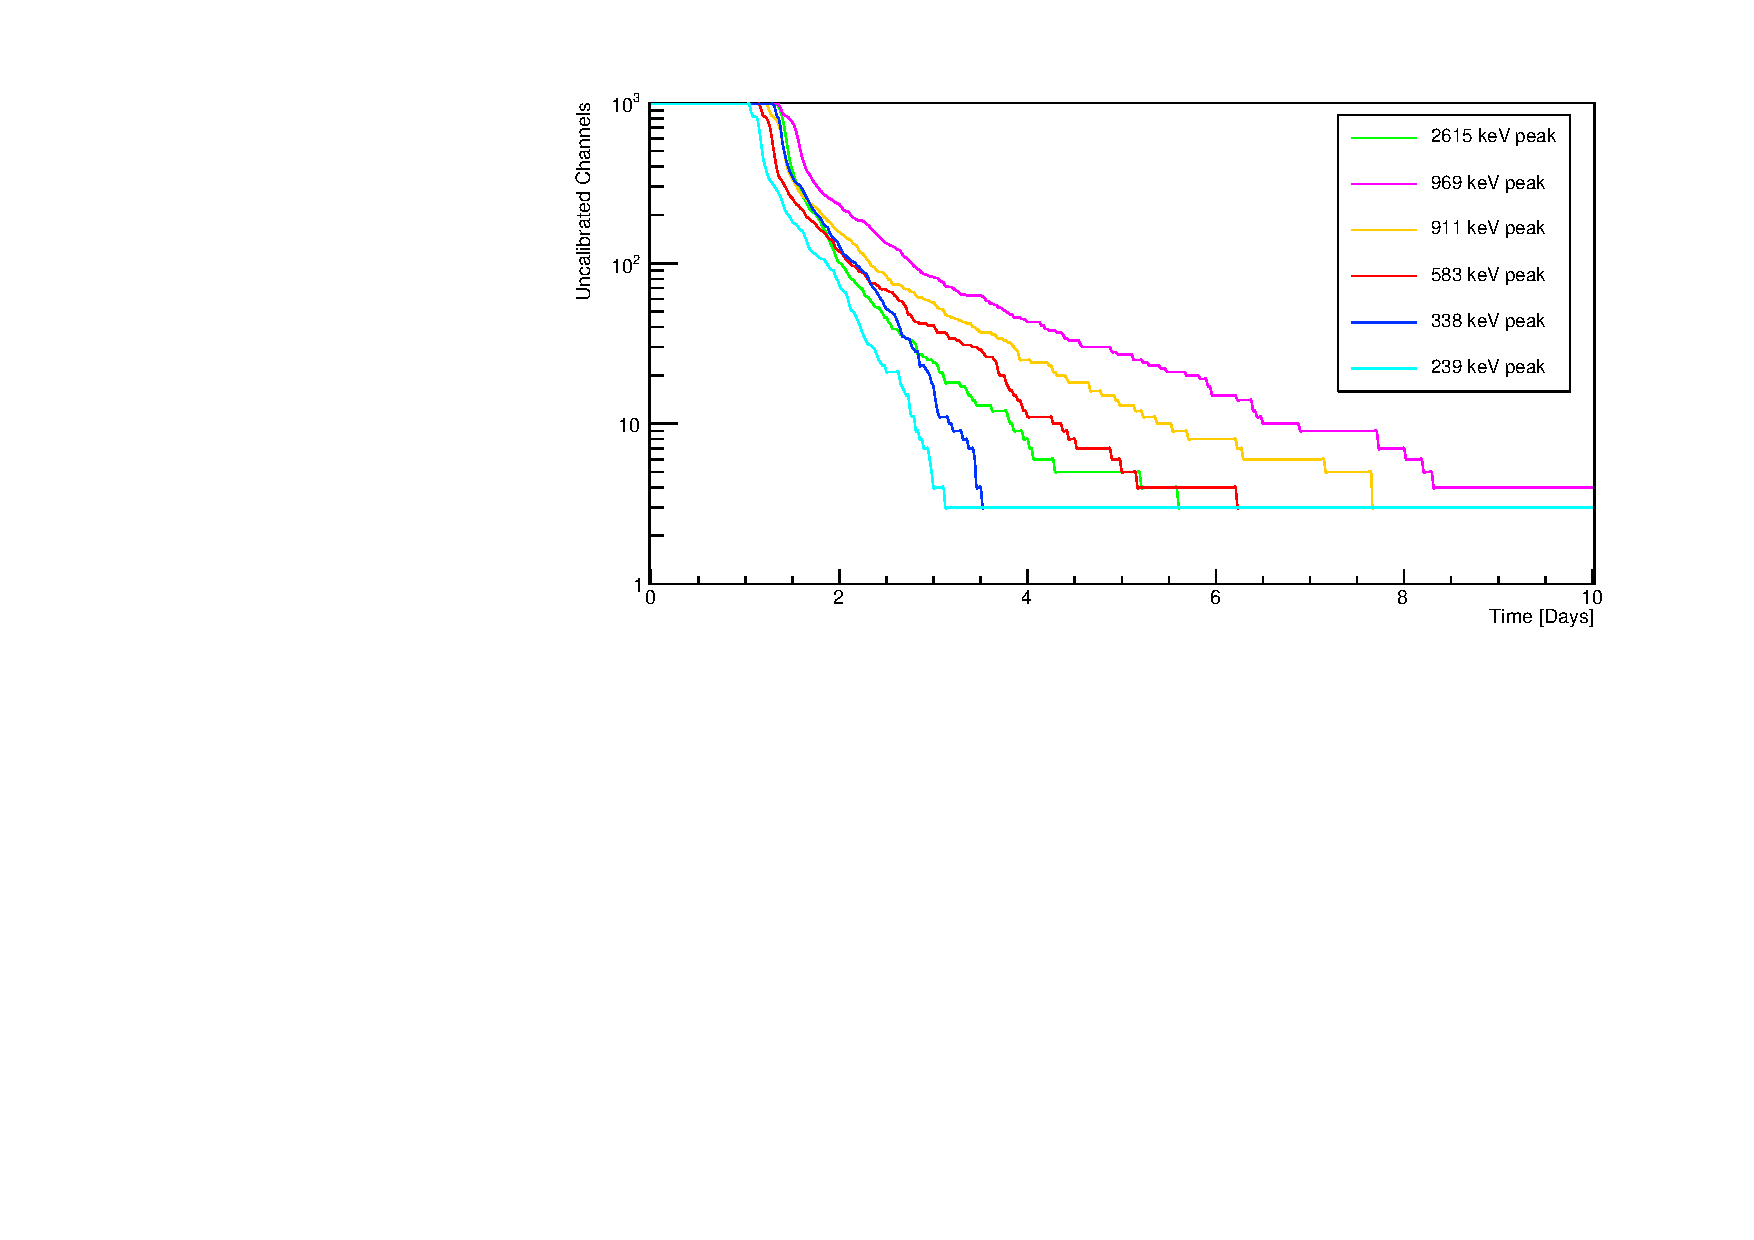
\includegraphics[width=\textwidth]{Figures/April2018_50counts.pdf}
\caption{}
\label{fig:april_calibration}
\end{subfigure}
\qquad
\begin{subfigure}[t]{0.9\textwidth}
\centering
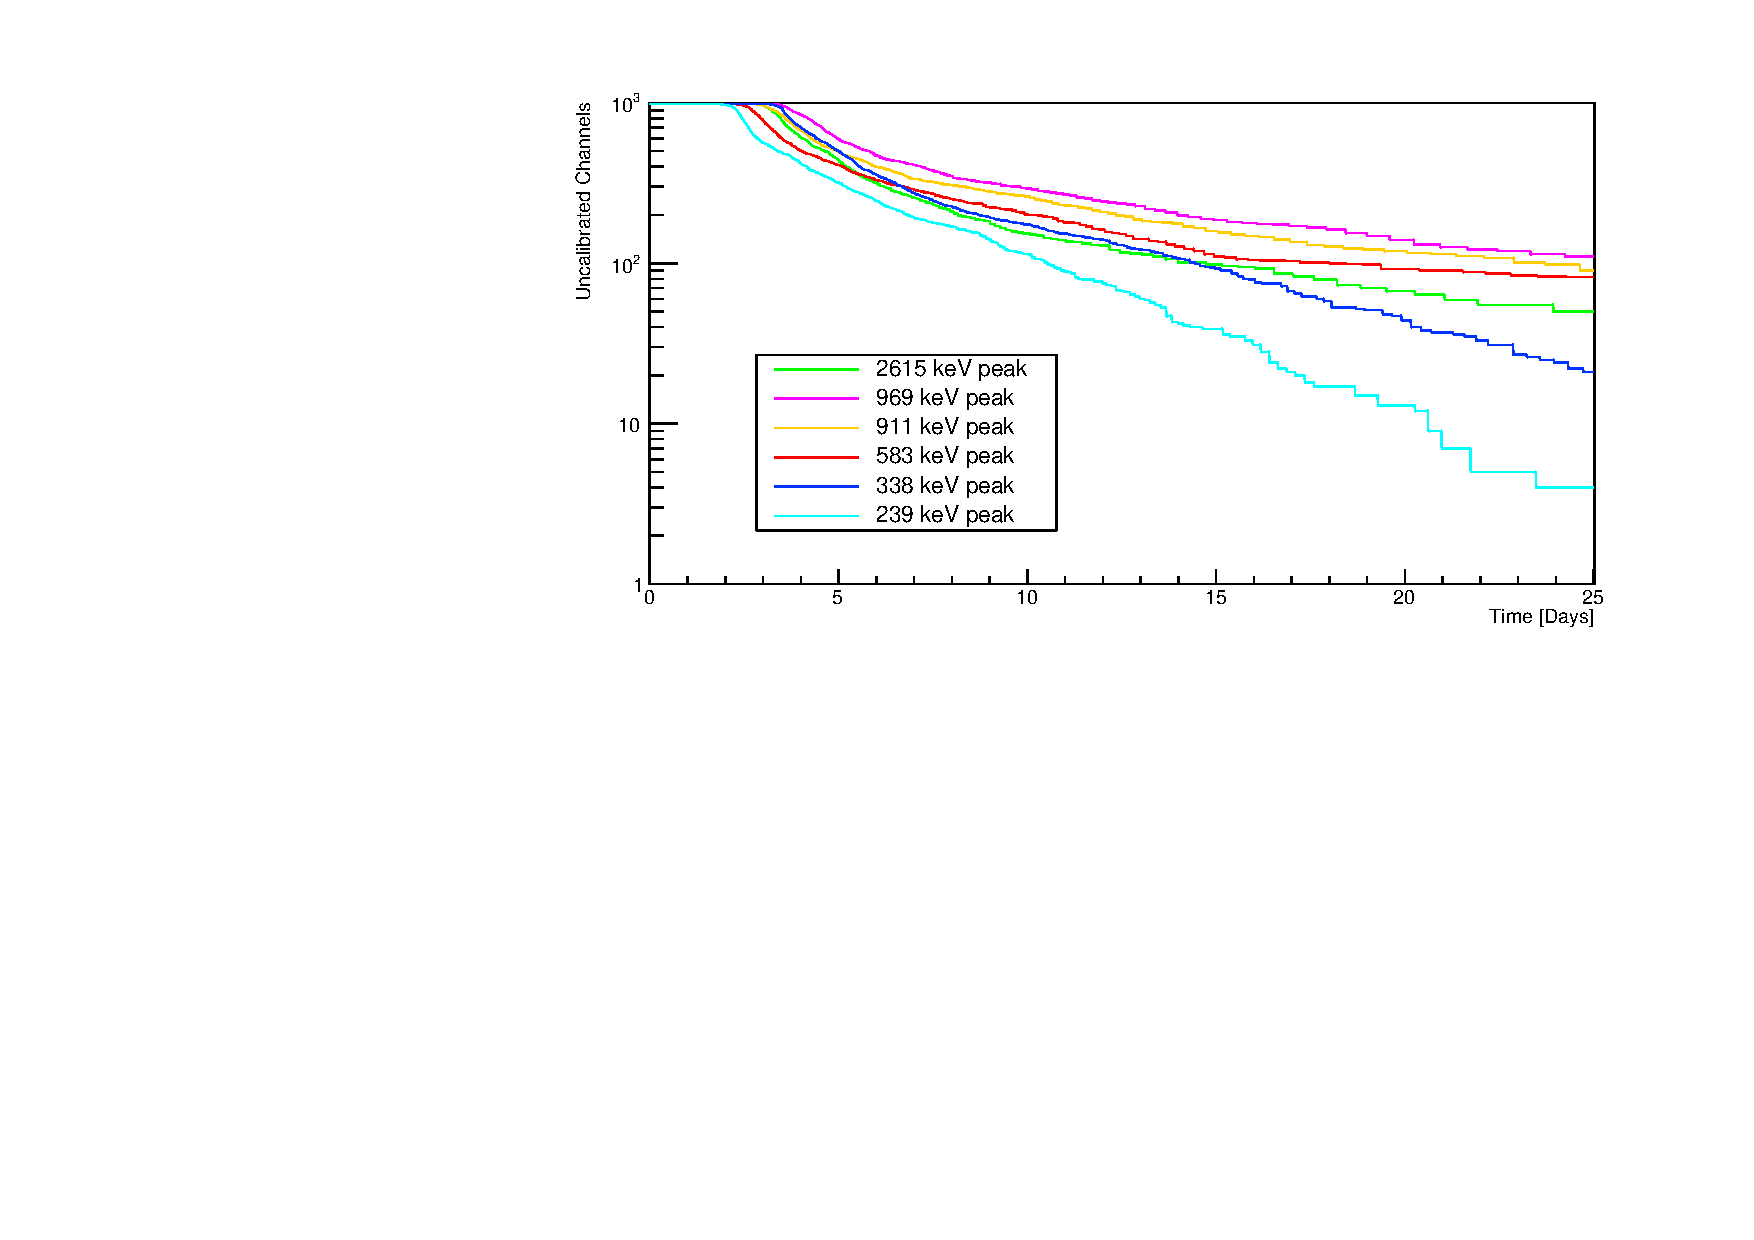
\includegraphics[width=\textwidth]{Figures/Sep2017_50counts.pdf}
\caption{}
\label{fig:september_calibration}
\end{subfigure}
\caption[Calibration times for April 2018 (a) and September 2017 (b) calibrations]
{Calibration times for April 2018 (a) and September 2017 (b) calibrations.
The calibration time considerably worsens depending on the state of the strings in cryostat.
For the calibration in April, 10 (5 inner, 5 outer) of the 12 DCS strings were able to be deployed into the cryostat, and for the calibration in September, only 5 (3 inner, 2 outer) strings were able to deploy successfully into the cryostat.
For comparison, the calibration times with the full system fully deployed is shown in \autoref{fig:FullString_50counts}.}
\label{fig:calibrations_50counts}
\end{figure}

Despite this at times, dismal performance of the system, the ability of the DCS to be able to have any success at all with such difficult technical challenges remains a significant accomplishment.
While these design flaws of the system are considerable and need to be overcome, the fact that radioactive sources can be brought down at all from room temperature to 10 mK is an impressive achievement.
The thermalization mechanisms, motor control, and software and hardware interlocks have performed well to conserve the system and keep it operating as long as possible, given the difficulties posed by these two issues.